% !TeX spellcheck = en_US
% !TeX encoding = UTF-8

% COMPILE WITH:
% `latexmk`
% You need lualatex and biber (in all TeXLive distributions)

\documentclass[
    numbers=noenddot,
    %listof=totoc,
    parskip=half-,
    fontsize=12pt,
    paper=a4,
    oneside,
    titlepage,
    bibliography=totoc,
    chapterprefix=false,
    captions=tableheading,
%    draft
]{scrbook}

% use lualatex or xelatex
%\usepackage{fontspec}
% Force real image rendering even if an editor recipe injects draft mode.
\usepackage[final]{graphicx}
\usepackage[onehalfspacing]{setspace}

% better language support
%\usepackage{polyglossia}
%\setdefaultlanguage{english}
%\setotherlanguage{german}

\usepackage{tocbasic}
\usepackage{booktabs}
\usepackage{multicol}
\usepackage{multirow}

\usepackage[]{scrlayer-scrpage}

% better bibliography (biblatex style)
% use biber to compile
\usepackage[citestyle=alphabetic, bibstyle=alphabetic, sorting=nyt, backend=biber, language=english, backref=true, maxcitenames=2]{biblatex}

% better quotes
% use \enquote{text}
\usepackage[autostyle,english=american,german=quotes]{csquotes}
\addbibresource{bibliography.bib}
\appto\bibsetup{\emergencystretch=1em}

% Float pages fill from the top instead of centering a lone figure or table.
\makeatletter
\setlength{\@fptop}{0pt}
\setlength{\@fpsep}{8pt plus 2fil}
\setlength{\@fpbot}{0pt plus 1fil}
\makeatother
\renewcommand{\topfraction}{0.85}
\renewcommand{\textfraction}{0.1}
\renewcommand{\floatpagefraction}{0.7}

% appendix
\usepackage[titletoc]{appendix}

% Self-contained manuscript assets for local, Prism, and Overleaf builds.
\graphicspath{{images/}}

% YOUR PACKAGES
\usepackage{amsmath}
\usepackage{amssymb}
\usepackage{array}
\usepackage{longtable}
\usepackage{tabularx}
\usepackage{listings}
\usepackage{microtype}
\usepackage{xurl}
\usepackage{seqsplit}
\usepackage{tikz}
\usetikzlibrary{positioning,arrows.meta,calc}
\usepackage[colorlinks=true, allcolors=blue]{hyperref}

\newcommand{\code}[1]{\texttt{#1}}
\newcommand{\hashvalue}[2]{\texttt{\seqsplit{#1#2}}}
\newcommand{\vect}[1]{\boldsymbol{#1}}
\lstset{
    basicstyle=\ttfamily\footnotesize,
    breaklines=true,
    columns=fullflexible,
    keepspaces=true,
    showstringspaces=false
}

% Registered title; personal and submission fields remain explicit blockers.
\title{Weakly Supervised Video Anomaly Understanding with Parameter-Efficient Adaptation and Temporal Grounding for Emergency Response}

% Author
\author{Pranav Maheshwari}

% Date
% Compile date as DD.MM.YYYY; used on the title page and in the declaration.
\date{\ifnum\day<10 0\fi\the\day.\ifnum\month<10 0\fi\the\month.\the\year}

% CHOOSE ACCORDINGLY
%\newcommand{\thesisType}{Bachelorarbeit}
\newcommand{\thesisType}{Masterarbeit}

\makeatletter
\let\thetitle\@title
\let\theauthor\@author
\let\thedate\@date
\makeatother

\pagestyle{scrheadings}

\begin{document}

%%%%%%%%%%%%%%%%%%%%%%%%%%%%%%%%%%%%%%%%%%%%%%%%%%%%%%%%%%%%%%%%%%%%%%%%%%%%%%%%%%%%%%%%%
\frontmatter
% CHOOSE ACCORDINGLY
%\include{includes/BA-titlepage}
% !TeX spellcheck = en_US
% !TeX encoding = UTF-8
\begin{titlepage}
    \centering
    \begin{onehalfspace}

        	
\includegraphics[width=7cm]{uni-logo.png}\\
        	\vspace{1.0cm}
	        	\large {\bfseries Lehrstuhl f\"ur Informatik und Mathematik}\\

        	\vspace{2.5cm}

            \begin{doublespace}
            	{\textsf{\Huge{\thetitle}}}
            \end{doublespace}

        	\vspace{2cm}

            \Large{Masterarbeit von}\\

        	\vspace{1cm}

        	{\bfseries \large{\theauthor}}

        	\vfill

        	{\large
        		\begin{tabular}[l]{c@{\hspace{1.5cm}}c}
			\textsc{1.~Pr\"ufer} & \textsc{2.~Pr\"ufer} \\
			{Dr.\ Mario D\"oller} & {Mohammadreza Mohebbi Najmabad}
        		\end{tabular}
        	}

        	\vspace{1.5cm}

        	\parbox{\linewidth}{\hrule\strut}

            \vfill

	    \thedate
    \end{onehalfspace}
\end{titlepage}


\tableofcontents
\newpage

% -- ABSTRACT
% !TeX spellcheck = en_US
% !TeX encoding = UTF-8
\chapter*{Abstract}
\markboth{Abstract}{Abstract}

This thesis builds and evaluates a weakly supervised pipeline that, for each
UCF-Crime video, decides whether it is anomalous, which of three
project-defined services (Police, Medical, Fire) it involves, and where the
event occurs. The pipeline combines VideoMAE with low-rank adaptation (LoRA),
frozen clip features, a normal-prototype distance, and an attention multiple
instance learning model with a binary head and a three-channel response head.
Each output is compared with a trivial reference on the same videos, and
Stage-2 training is repeated with three seeds over a fixed feature store.

Video-level binary detection was stable: on fixed 16-clip test bags, the area
under the receiver operating characteristic curve was $0.940\pm0.002$ (mean
$\pm$ standard deviation over the three Stage-2 seeds), a video-level value
that is not comparable with frame-level UCF-Crime results. Response selection
was weak. Without gating the head predicted Police for every video, and after
binary gating it exceeded a rule that predicts every service for each detected
anomaly by only 0.015 in Macro-F1 (95\% video bootstrap interval 0.008 to
0.023). A validation-only extension that added normal bags to the response loss
removed the universal Police output, but its gated margins stayed within the
seed spread of the control. On a dense protocol covering 99.843\% of test-video
frames, attention reached a temporal average precision of $0.327\pm0.014$ and
an interval overlap of $0.186\pm0.017$, above trivial references but far from
precise localization.

The contribution is an offline implementation and a matched evaluation that
keeps anomaly detection, response prediction, and temporal grounding separate.
The response targets are deterministic transformations of dataset categories
rather than observed service decisions, and the computer-aided dispatch
(CAD)-style output has no calibration, safety, or operational validation.

\newpage

% -- Acknowledgements
% !TeX spellcheck = en_US
% !TeX encoding = UTF-8
\chapter*{Acknowledgments}
\markboth{Acknowledgments}{Acknowledgments}

The completion of this thesis is an important milestone for me, both academically and personally. It would not have been possible without the support of many people, and I would like to express my sincere gratitude to everyone who contributed with their patience, guidance, and encouragement.

First, I thank my first examiner, Dr.\ Mario D\"oller, for his time, his assessment of this work, and his valuable feedback. I am equally grateful to my supervisor, Mohammadreza Mohebbi Najmabad, for his continuous guidance and constructive criticism. His advice on the structure, the evaluation, and the presentation of this work improved it considerably.

I also thank the University of Passau and the department for providing an excellent academic environment throughout my master's studies. The knowledge and skills I gained there laid the foundation for this thesis.

I am grateful to the open-source community. This work relies on freely available software and research, including PyTorch, Hugging Face Transformers, PEFT, NumPy, SciPy, scikit-learn, Matplotlib, and OpenCV. I also thank the authors of the cited publications and of the UCF-Crime dataset for making their work available.

Last, I thank my friends and family for their constant support, understanding, and encouragement throughout my studies. Their help during this period meant a great deal to me.

\newpage

% -- List of figures
\thispagestyle{empty}
\cleardoublepage
\listoffigures
\newpage

% -- List of tables
\thispagestyle{empty}
\cleardoublepage
\listoftables
\newpage

%%%%%%%%%%%%%%%%%%%%%%%%%%%%%%%%%%%%%%%%%%%%%%%%%%%%%%%%%%%%%%%%%%%%%%%%%%%%%%%%%%%%%%%%%
\mainmatter

% -- Chapters
% following IMRaD structure
% adjust for your liking
% !TeX root = ../thesis.tex
\chapter{Introduction}
\label{chap:introduction}

\section{Motivation}
\label{sec:introduction-motivation}

Long, untrimmed surveillance video presents a difficult allocation problem: most
recorded time is routine, while events that warrant review may be brief, visually
ambiguous, and separated by long periods of normal activity. Automated video
analysis can help prioritize where a person looks, but an anomaly score alone is
not an emergency-response decision. A useful research account must distinguish
at least three questions: whether a video is anomalous, what kind of response a
predefined label scheme associates with it, and where the supporting event occurs
in time. Conflating these questions can make a strong detector appear to be a
capable response system even when its service selection or temporal grounding is
weak.

UCF-Crime made this setting accessible at scale by collecting 1,900 long,
untrimmed surveillance videos, including normal activity and 13 anomaly
categories, and by defining both binary anomaly detection and anomalous-activity
recognition tasks \cite{sultani2018real}. Its training supervision is available
at video level rather than as clip-level event labels. This reduces the need for
dense training annotation, but creates ambiguity: an anomalous video can contain
many normal clips, and its category does not identify which clips depict the
event. Weakly supervised video anomaly detection therefore has to learn from
bags of temporally mixed evidence rather than from precisely labeled instances.

The application framing raises a second difficulty. A camera record does not by
itself specify whether Police, Medical, Fire, some other service, or no immediate
service is appropriate. Such a decision depends on context that may not be
visible in the video and on institutional, legal, and professional judgment.
Research on semi-automated closed-circuit television (CCTV) has also shown that
system accuracy, confidence information, task complexity, and interface design
affect operator reliance and workload \cite{dadashi2013semiautomated}. For this
reason, response-oriented outputs should be evaluated as decision-support
signals with explicit human oversight, not presented as automatic dispatch.

The goal of this thesis is to build and evaluate a weakly supervised pipeline
that answers all three questions for UCF-Crime videos, and to measure each
answer separately against simple references. In the registered title,
\emph{understanding} therefore means three measurable outputs: a binary anomaly
decision, a set of project-defined response labels, and the temporal alignment
of attention with annotated events. \emph{Emergency response} names the
application framing of an offline system; it is not an operationally validated
capability.

\section{Problem Statement and Research Gap}
\label{sec:introduction-gap}

Weakly supervised video anomaly detection is commonly formulated with multiple
instance learning (MIL): a video is a bag, temporal snippets are instances, and
only the bag label is known during training \cite{sultani2018real,tian2021weakly}.
This formulation supports video-level learning and can produce snippet scores,
but success at one level does not establish success at another. A high video
area under the receiver operating characteristic curve (AUROC) does not
guarantee balanced recognition of anomaly categories, selective
multi-label response prediction, or accurate event boundaries. Likewise, a
visually plausible attention trace is not automatically a calibrated anomaly
probability or a faithful explanation of a decision.

Three methodological strands are relevant but remain conceptually distinct.
First, pretrained video representations can reduce the amount of task-specific
learning required; VideoMAE learns spatio-temporal representations through
masked video reconstruction \cite{tong2022videomae}. Low-rank adaptation (LoRA)
offers a parameter-efficient way to adapt selected projections while leaving the
pretrained weights frozen \cite{hu2021lora}. Second, MIL aggregation and
normality-oriented memories can prioritize instances when only bag labels are
available \cite{ilse2018attention,zhou2023ur}. Third, independent sigmoid outputs
and imbalance-aware objectives support non-exclusive labels
\cite{boutell2004learning,ridnik2021asymmetric}. Combining these elements in
software is not itself evidence that each element is beneficial, nor that their
outputs form a reliable integrated response system.

Published weakly supervised methods on UCF-Crime are compared mainly through
a single number, the frame-level AUC of an anomaly score
(Section~\ref{sec:background-comparison}). Three things are rarely reported
together with it: an output that states which services an event involves, a
per-video measurement of where the event is placed in time, and a comparison
of each learned output with a trivial rule on the same videos. Without such
references, a strong detector can look like a capable response system without
showing whether a rule that predicts every service after the same anomaly
decision would do as well. This thesis addresses that evaluation gap. It implements one sequential
pipeline that adapts a video encoder, freezes clip features, adds a
normal-prototype distance, trains an attention MIL model with a binary head and
three response channels, and renders an offline computer-aided dispatch
(CAD)-style record. It then evaluates the binary, response, and temporal outputs
separately, each against a matched reference, across repeated Stage-2 training.

\section{Research Questions}
\label{sec:introduction-rqs}

The following four questions define the empirical scope of the thesis:

\noindent\textbf{RQ1:} \emph{What video-level binary anomaly-detection
performance does the sequential LoRA–\allowbreak prototype–\allowbreak MIL pipeline achieve on
UCF-Crime under weak video-level supervision?}

\noindent\textbf{RQ2:} \emph{On UCF-Crime, what limitations are evident in the
reconciled historical 14-class predictions, and what error profile does the
project-defined multi-label emergency-response formulation exhibit?}

\noindent\textbf{RQ3:} \emph{How stable are binary and project-defined
response-channel predictions across Stage-2 training seeds under fixed feature
and evaluation artifacts on UCF-Crime, and how do matched response-label error
metrics differ with and without binary gating?}

\noindent\textbf{RQ4:} \emph{To what extent do the final checkpoints’ attention
outputs align with annotated anomalous intervals under the dense indexed-video
UCF-Crime evaluation protocol?}

RQ2 also covers an earlier 14-class formulation of the same pipeline, which is
reported as development history (Section~\ref{sec:results-historical}). RQ1
concerns the complete sequential configuration as executed, while its
reported variability is conditional on the frozen representation and prototype
artifacts. RQ2 describes two non-equivalent tasks separately and does not define
a before-and-after performance comparison. RQ3 treats gating as a matched
computational transformation of response-label predictions, not as evidence of
real dispatch effectiveness. RQ4 includes all three final checkpoints and uses
attention only as a temporal saliency signal whose overlap with annotations must
be measured.

\section{Scope and Contributions}
\label{sec:introduction-contributions}

The work makes an implementation-and-evaluation contribution. It does not claim
to invent VideoMAE, LoRA, MIL, attention pooling, asymmetric loss, or CAD. Its
contributions are as follows:

\begin{enumerate}
    \item \textbf{A sequential weakly supervised implementation.} The pipeline
    links video indexing and clip preparation, LoRA adaptation of VideoMAE,
    frozen adapted features, a normal-prototype distance, guided bag
    construction, and a shared-attention MIL model with a binary head and three
    response channels. It also supports dense indexed evaluation and
    deterministic offline CAD-style output. The stages are trained one after
    another, not jointly from pixels.

    \item \textbf{A separated evaluation design.} Historical 14-class outputs,
    validation-only studies, fixed-bag test results, and dense indexed results
    are reported separately. Fixed manifests, three Stage-2 seeds, per-video
    records, matched populations, trivial baselines, and hash-identified local
    artifacts keep positive and negative findings traceable.

    \item \textbf{A matched characterization of system behavior.} The response
    head is compared with predicting every service, with and without the same
    binary gate. The attention signal is compared with whole-video, uniform,
    random, and prototype-distance references, and alignment is measured per
    video under near-complete indexed coverage. Two validation-only studies, one
    on the prototype score with guided sampling and one on normal bags in the
    response loss, support the reading of these comparisons.

    \item \textbf{Explicit operational boundaries.} The thesis separates
    derived response labels from observed emergency decisions, temporal saliency
    from explanation, source-video timestamps from compute latency, and an
    offline record from a live CAD connection. These limits define what the
    evidence can support.
\end{enumerate}

The scope follows from these choices. UCF-Crime is used because it combines
real surveillance footage, named incident categories, weak training labels, and
annotated test intervals (Section~\ref{sec:background-tasks}). The Police,
Medical, and Fire targets are deterministic project transformations of its
categories, not observed service assignments. Only Stage-2 training is repeated
across three seeds; the adapted feature store and prototype memory remain fixed.
Temporal evaluation measures alignment with annotated intervals, not causal
explanation or real-time localization. All conclusions are restricted to
UCF-Crime, the fixed splits and artifacts, and the executed protocols; the work
does not establish generalization to other sites, calibration, real-time
throughput, human-factors performance, safety, or deployment readiness.

\section{Thesis Structure}
\label{sec:introduction-structure}

Chapter~\ref{chap:background} develops the concepts needed to read the method
and evidence: UCF-Crime supervision, task boundaries, MIL, video representation
learning, LoRA, prototype guidance, attention pooling, multi-label prediction,
gating, and temporal metrics, and closes with a comparison of related
approaches. Chapter~\ref{chap:methods}
specifies the implemented pipeline, data identities, objectives, evaluation
paths, and reproducibility limits. Chapter~\ref{chap:results} reports the
historical, fixed-bag, validation-only, dense indexed, and temporal results
without extending them into deployment claims. Chapter~\ref{chap:discussion}
answers RQ1--RQ4, interprets the error profiles, and addresses limitations,
ethics, human oversight, and future work. Chapter~\ref{chap:conclusion}
provides the final synthesis of the evidence and its bounded contribution.

% !TeX root = ../thesis.tex
\chapter{Background and Related Work}
\label{chap:background}

This chapter develops the concepts needed to interpret the implemented pipeline
and its evidence. The organization is thematic: it begins with the supervision
and task distinctions created by UCF-Crime, then connects MIL, video representation learning, parameter-efficient adaptation,
prototype guidance, response-label prediction, and temporal grounding. The
human-oversight and deployment implications these ideas raise are addressed
together with the evidence in Chapter~\ref{chap:discussion}, where they can be
grounded in measured failure modes rather than anticipated in the abstract.
The aim here is not to catalogue every video anomaly method. It is to make
clear which established ideas the thesis combines, what each idea can support,
and which conclusions still require direct evaluation.

\section{Video Anomaly Tasks under Weak Supervision}
\label{sec:background-tasks}

\subsection{UCF-Crime and Long Untrimmed Video}

An anomaly is meaningful only relative to a context and an expected range of
behavior. Chandola et al. define anomaly detection as finding patterns that do
not conform to expected behavior, and they describe contextual anomalies, which
are anomalous in one context but normal in another \cite{chandola2009anomaly}.
In surveillance video, the same visual action can be routine in one
location and concerning in another. The learning problem is therefore not a
closed catalogue of every possible abnormal event. It is a decision problem
defined by a dataset, its labels, and the operating context represented by its
cameras. This dependence is especially important when model inputs include
background, viewpoint, compression, and scene layout as well as the event of
interest.

UCF-Crime was introduced to move anomaly detection toward long, untrimmed,
real-world surveillance recordings. The dataset contains 1,900 videos totaling
approximately 128 hours, with normal videos and 13 anomaly categories such as
Abuse, Arson, Burglary, RoadAccidents, Robbery, and Shooting
\cite{sultani2018real}. The authors presented two uses: binary anomaly detection,
where the anomaly categories form one positive group, and anomalous-activity
recognition, where the individual categories are distinguished. For the
anomalous test videos, the authors also provide temporal annotations, the start
and end frames of each event, obtained by averaging the labels of several
annotators. These
facets make the dataset suitable for asking different questions, but they do not
make the answers interchangeable.

The videos are untrimmed: an anomalous video can begin and end with normal
activity, and the event may occupy only a small part of its duration. A
video-level anomaly label therefore states that relevant evidence occurs
somewhere in the video; it does not state that every sampled clip is anomalous.
Similarly, attaching the video's category to a sampled clip is a weak training
approximation rather than a verified clip annotation. This distinction matters
for both representation adaptation and downstream MIL. Treating inherited clip
labels as fully observed ground truth would conceal the central uncertainty of
the task.

Video anomaly detection has been approached with different amounts of
supervision. One line of work learns from regular video alone; Hasan et al., for
example, learn a generative model of regular motion patterns with an
autoencoder \cite{hasan2016learning}. Weakly supervised methods instead train
on video-level labels of both normal and anomalous videos, as in the ranking
approach of Sultani et al. discussed in Section~\ref{sec:background-mil}.
The two settings use different benchmarks (Table~\ref{tab:datasets}). UCSD
Ped1/Ped2 \cite{mahadevan2010anomaly}, CUHK Avenue \cite{lu2013abnormal}, and
the ShanghaiTech Campus dataset \cite{liu2018future} were built for the
normal-only setting. Their anomalies are mostly local deviations such as
vehicles among pedestrians, running, or loitering. Each video comes from one of a
few fixed scenes, and the standard training split contains no
anomalies. Zhong et al.\ later reorganized ShanghaiTech into a weakly
supervised split of 238 training and 199 test videos \cite{zhong2019graph}, but
its anomaly types remain unnamed. XD-Violence is larger and weakly labeled, but
it mixes movies, sports, games, and hand-held recordings with surveillance
footage and centers on violence with audio \cite{wu2020not}.

UCF-Crime is the only one of these benchmarks that combines four properties
this thesis needs: real surveillance footage from many scenes, named incident
categories from which a response mapping can be derived, weak video-level
labels for training, and frame-level annotations of the anomalous test videos.
It is also the benchmark on which most of the weakly supervised methods compared
in Section~\ref{sec:background-comparison} report results.

\begin{table}[!ht]
    \centering
    \small
    \caption[Video anomaly datasets.]{Video anomaly datasets as described by their authors or, for UCSD, Avenue, and ShanghaiTech, by Liu et al.\ \cite{liu2018future}. ``Normal only'' means that the standard training split contains no anomalies.}
    \label{tab:datasets}
    \begin{tabularx}{\textwidth}{@{}l l >{\raggedright\arraybackslash}X l@{}}
        \toprule
        \textbf{Dataset} & \textbf{Videos (train / test)} & \textbf{Content and anomaly types} & \textbf{Training labels} \\
        \midrule
        UCSD Ped1 \cite{mahadevan2010anomaly} & 34 / 36 & Pedestrian scene; 40 events, vehicles such as bicycles and cars & Normal only \\
        UCSD Ped2 \cite{mahadevan2010anomaly} & 16 / 12 & Pedestrian scene; 12 events, same definition & Normal only \\
        CUHK Avenue \cite{lu2013abnormal} & 16 / 21 & One scene; 47 events such as throwing, loitering, running & Normal only \\
        ShanghaiTech \cite{liu2018future} & 330 / 107 & 13 scenes; 130 events of various, uncategorized types & Normal only \\
        UCF-Crime \cite{sultani2018real} & 1,610 / 290 & Real surveillance, 128\,h; 13 named crime and accident categories & Video level \\
        XD-Violence \cite{wu2020not} & 3,954 / 800 & Movies, web, and CCTV with audio, 217\,h; 6 violence types & Video level \\
        \bottomrule
    \end{tabularx}
\end{table}

A more recent direction brings in language. VadCLIP adapts a frozen CLIP
(Contrastive Language--Image Pre-training) model
with two branches, one for coarse binary classification and one that aligns
video features with textual category labels \cite{wu2024vadclip}. Anomize
targets open-vocabulary detection, in which anomaly categories not seen during
training must still be detected and named \cite{anomize2025cvpr}. UCA annotates
UCF-Crime with sentence-level event descriptions and their timing to study
surveillance video-and-language understanding \cite{yuan2024surveillance}, and, in a preprint,
Holmes-VAD fine-tunes a multimodal large language model to explain the
anomalies it detects \cite{zhang2024holmes}. In these works, understanding
means describing or naming an event in language. The pipeline in this thesis
takes a narrower route. It uses visual features only, produces no free-text
description, and predicts a fixed vocabulary of three response channels, so its
use of the term is limited to a video-level anomaly decision, response
channels, and temporal support. It also runs offline on stored videos, whereas
Karim et al. train a weakly supervised detector end to end for real-time
decisions \cite{realtime2024wacv}.

In this thesis, UCF-Crime is consequently both the empirical domain and a scope
boundary. Its video identities, fixed split, categories, and temporal annotations
define the reported questions. The dataset does not supply Police, Medical, or
Fire decisions, and it does not establish generalization to a new camera network
or institution. For the present work, this means that UCF-Crime supports weakly supervised video-level learning and test-time temporal
measurement, but response labels must be identified as a separate,
project-defined transformation.

\subsection{Detection, Classification, and Temporal Localization}

Three output levels recur throughout this thesis. \emph{Binary anomaly
detection} assigns a video, or sometimes a temporal unit within it, to Normal or
Anomaly. At video level, the output answers whether the recording contains an
event from the dataset's anomaly group. A score can be evaluated without fixing
a decision threshold through AUROC, which equals the probability that a randomly
chosen positive is ranked above a randomly chosen negative
\cite{fawcett2006introduction}. Precision, recall, and F1 instead require a
decision rule. When negatives greatly outnumber positives, a ROC curve can look
favorable while many false positives remain, and precision--recall analysis
gives the more informative picture
\cite{davis2006relationship,saito2015precision}. The distinction matters here
because the video-level test split is nearly balanced, with 140 anomalous and
150 normal videos, whereas annotated anomalous frames usually cover only part
of a video.

\emph{Anomaly classification} assigns semantic labels. The historical task in
this thesis is single-label 14-class classification: Normal plus the 13
UCF-Crime anomaly categories form mutually exclusive outcomes. The later
response task is different. It predicts three non-exclusive channels and can
activate more than one at a time. A macro-averaged F1 score (Macro-F1) from the
14-class softmax problem is therefore not commensurate with a Macro-F1 value
averaged over three
binary response channels. Label spaces, losses, thresholds, supports, and error
opportunities all differ.

\emph{Temporal localization} asks where an event occurs. It requires evidence
at a finer temporal resolution than the video label. In weakly supervised video
anomaly detection, snippet scores or pooling weights may be projected back to
time even though interval labels were not used for training. This produces a
measurable temporal signal, but one that should be evaluated explicitly against
annotations. Video-level correctness alone cannot establish accurate event
boundaries, because a model may classify a video from scene context or attend to
only a small, displaced part of the event.

These tasks form a hierarchy of questions, not a hierarchy of guaranteed
capabilities. A correct binary decision can coexist with the wrong semantic
label; a correct response vector can coexist with a temporally displaced
interval; and a localized high score can coexist with a wrong video decision.

\section{Multiple Instance Learning for Weakly Labeled Video}
\label{sec:background-mil}

\subsection{Bags, Instances, and Ambiguous Positive Evidence}

Multiple instance learning names exactly this situation: one labeled bag
contains several instances, and the instance responsible for a positive label
is unknown \cite{dietterich1997solving}. Its classical assumption is binary --
a positive bag holds at least one positive instance, a negative bag holds none
-- and modern neural MIL keeps that separation between bag-level supervision
and latent instance relevance even as it relaxes the original geometric model.

For video anomaly detection, a complete video becomes a bag and clips or
snippets become its instances. Normal videos provide negative bags, whereas an
anomalous video provides a positive bag with an unknown mixture of normal and
anomalous temporal content. Sultani et al. used this view to learn an anomaly
ranking function from video-level labels, comparing high-scoring instances from
anomalous and normal bags while adding sparsity and temporal smoothness
constraints \cite{sultani2018real}. The formulation directly addresses the
annotation problem: it does not require the anomalous segment to be labeled
during training.

Later weakly supervised approaches illustrate why instance selection and
representation quality are coupled. The Multiple Instance Self-Training
framework (MIST) alternates MIL-based pseudo-label
generation with refinement of task-specific video representations
\cite{feng2021mist}. Robust Temporal Feature Magnitude learning (RTFM) focuses on
feature magnitudes and selects discriminative
instances while modeling temporal dependencies \cite{tian2021weakly}. These
approaches differ in architecture and objective, but both address a common
difficulty: the normal snippets that dominate an anomalous video's duration can
overwhelm the comparatively rare positive evidence.

Other weakly supervised methods select or correct instance evidence in
different ways. RTFM ranks snippets by feature magnitude, and MGFN (Magnitude-Contrastive
Glance-and-Focus Network) keeps
magnitudes but adds a magnitude-contrastive loss, motivated by the observation
that feature magnitudes are inconsistent across scenes
\cite{tian2021weakly,chen2023mgfn}. Zhong et al. treat the weak labels as noisy
snippet labels, clean them with a graph convolutional network, and then train a
supervised action classifier \cite{zhong2019graph}. CLAWS (Clustering Assisted
Weakly Supervised Learning with normalcy Suppression) combines a
normalcy-suppression mechanism, which lowers the anomaly scores of normal
regions, with a clustering-distance loss that separates normal and anomalous
representations \cite{zaheer2020claws}. Li et al. use sequences of several
snippets instead of single snippets as the unit of selection and refine the
snippet scores by self-training with a transformer \cite{li2022self}. The
attention pooling described in the next subsection ranks instances by learned
weights rather than by feature magnitude, and in the binary pool every instance
keeps a non-negative weight. The VadCLIP authors also note that most current
methods operate on features precomputed by a pretrained extractor such as I3D
(Inflated 3D ConvNet)
\cite{wu2024vadclip,carreira2017quo}; the pipeline here likewise works on stored
clip features.

The bag assumption is useful but imperfect for surveillance video. A video-level
category may be uncertain, the event may be visually subtle, and a nominally
normal video cannot enumerate every acceptable behavior. MIL also does not by
itself specify how to aggregate evidence, how many instances to sample, or how
to handle a positive bag in which selected clips miss the event. Those choices
become part of the method and must be assessed under the actual sampling
protocol.

MIL therefore supplies the correct abstraction for weak video labels, but
not a guarantee of instance discovery. Fixed-size training bags, fixed-bag
evaluation, and dense variable-length evaluation expose different subsets of
the temporal evidence. Their results must therefore be named by input protocol
rather than treated as interchangeable measurements of one abstract model.

\subsection{Pooling, Attention, and Top-Instance Selection}

A MIL model requires a permutation-invariant operation that converts a set of
instance representations into a bag representation. Maximum pooling embodies a
strong positive-instance assumption: the most activated instance determines the
bag. Mean pooling distributes influence across all instances, which can suppress
a brief event when normal content dominates. Top-$k$ pooling lies between these
extremes by using a selected subset, but its behavior depends on both $k$ and the
ranking function.

Attention-based MIL learns non-negative instance weights that sum to one and
forms a weighted bag representation -- a trainable, permutation-invariant
alternative to fixed pooling operators \cite{ilse2018attention,zaheer2017deep}.
The weights identify which instances contribute most to the aggregate and
accommodate bags of different sizes, without requiring an externally specified
positive clip during training.

Attention pooling and top-instance pooling answer related but different needs.
The weighted mean gives the classifier a differentiable global summary. A
top-attention subset allows a second branch to retain high-ranked instances and
combine statistics such as their element-wise maximum and mean. Maximum values
can preserve a strong feature response, while the mean describes what is shared
across the selected subset. Concatenating these statistics with the attention
pool provides more than one view of a bag without claiming that any individual
view is sufficient.

Softmax attention is also only relative within a bag: adding instances changes
the normalizing denominator and can shift every weight even when one clip's
representation is unchanged, so a threshold applied after per-video smoothing
is not a global probability threshold. The same effect scales the top-quarter
selection rule from four clips in a 16-instance training bag to many more
clips in dense evaluation, from the identical checkpoint.

The implementation studied here uses one shared attention scorer for binary
pooling and for ranking instances used by the response branch. This reuses a
common temporal ordering, but it does not prove that the ordering is optimal
for both tasks.

\section{Video Representation Learning and Parameter-Efficient Adaptation}
\label{sec:background-representation}

\subsection{VideoMAE Representations}

Video inputs contain appearance and motion across space and time. A clip encoder
must transform that high-dimensional signal into a representation that can be
stored, sampled, and aggregated. Transformer-based video encoders divide a clip
into spatio-temporal tokens and use self-attention layers to model relations
among them. The design follows the Transformer \cite{vaswani2017attention} and
its application to images as sequences of patches in the Vision Transformer
\cite{dosovitskiy2020image}. The output can remain token-level for fine spatial
reasoning or be pooled into one vector per clip for downstream temporal
modeling.

VideoMAE learns such representations through masked autoencoding
\cite{tong2022videomae}: during self-supervised pretraining it masks a high
proportion of spatio-temporal tube tokens and reconstructs the missing content,
exploiting temporal redundancy to force the encoder toward structure that
survives reconstruction. The published model is a general video representation
learner; it does not encode the UCF-Crime response mapping or the evaluation
protocol used in this thesis.

Using a pretrained clip encoder separates two learning problems. The encoder
maps pixels to features, while the MIL model learns how to combine features
across a video. This separation can make long-video experiments tractable
because clip embeddings are extracted once and reused. It also creates a strong
provenance dependency: after features are frozen, later experiments are
conditional on the exact encoder checkpoint, preprocessing, software loader,
sampling choices, and stored feature identities.

The pipeline uses globally averaged VideoMAE token states rather than retaining
patch-level tokens. This provides a compact clip representation for MIL, but
removes the information needed for spatial localization within a frame. Dense
temporal sampling can improve coverage along the time axis; it cannot recreate
discarded spatial tokens.

\subsection{Low-Rank Adaptation}

Full fine-tuning updates every parameter of a pretrained encoder, at a
corresponding optimizer-state and storage cost. LoRA avoids that cost by
freezing the pretrained weight matrix and representing its task-specific
update as the product of two trainable low-rank matrices instead
\cite{hu2021lora}. If a frozen projection is
$W_0$, the adapted projection has the form
\begin{equation}
    W' = W_0 + \frac{\alpha}{r}BA,
\end{equation}
where $r$ is the chosen rank and $A$ and $B$ are the trainable factors. When
$r$ is much smaller than the input and output dimensions, the number of
trainable parameters is substantially smaller than for a dense update.

LoRA is one of several parameter-efficient alternatives to full fine-tuning.
Adapter modules insert small trainable layers into a frozen network
\cite{houlsby2019parameter}, and ST-Adapter, AIM, and AdaptFormer use such
modules to transfer pretrained image transformers to video or to adapt
pretrained vision transformers to new recognition tasks
\cite{pan2022st,yang2023aim,chen2022adaptformer}. Prompt tuning takes a
different route and learns a small set of input tokens while the backbone stays
frozen \cite{lester2021power,jia2022visual}. He et al. show that several of
these methods can be described as modifications of specific hidden states of
the pretrained model \cite{he2022towards}. No comparison among these
alternatives was run for this thesis; LoRA was a design choice, and its
selection is not a result.

LoRA was introduced for large language models, so applying it to a video
transformer is a transfer of an adaptation mechanism rather than a new LoRA
method. The practitioner must still choose which projections receive adapters, the rank,
scale, dropout, optimization schedule, and selection criterion. Parameter
efficiency does not imply compute-free adaptation, and a small trainable subset
does not guarantee better generalization than frozen features or full
fine-tuning.

In a sequential pipeline, adapter selection also precedes downstream evidence.
Once the adapted encoder is frozen and the feature store is extracted, the MIL
model cannot correct the encoder through pixel-level gradients. Conversely,
repeating only MIL training does not measure variation in adapter training. A
three-seed MIL result over one feature store is therefore narrower than a
three-seed repetition of the whole pipeline.

For this thesis, LoRA has a limited and defensible rationale: it provides a
parameter-efficient task-adaptation stage before frozen feature extraction. The
final results evaluate the executed LoRA--prototype--MIL sequence, but there is
no matched test experiment that isolates a causal performance gain from LoRA.
This boundary is essential to the interpretation of RQ1.

\section{Normal Prototypes and Guided Instance Sampling}
\label{sec:background-prototypes}

Distance from a representation of normality is a recurring idea in anomaly
detection. A single global center can be too restrictive when routine behavior
has several modes, while a set of prototypes can summarize multiple regions of
the normal feature space. A clip far from its nearest normal prototype may be
unusual under that representation, although distance alone does not reveal the
semantic cause or prove that the clip is anomalous.

Prototype memories have also appeared in weakly supervised video anomaly
detection. Uncertainty Regulated Dual Memory Units (UR-DMU) learns normal and
abnormal memory units and uses them to
separate feature structure under weak supervision \cite{zhou2023ur}. The present
pipeline makes a narrower construction. It clusters only embeddings from normal
training videos, then defines a clip score by squared distance to the nearest
normal center. It does not reproduce the dual-memory architecture, uncertainty
regulation, or training objective of UR-DMU.

The distance can affect learning in two conceptually separate ways. As an
appended scalar feature, it lets the MIL model decide whether distance is useful
alongside the clip embedding. As a sampling guide, it increases the chance that
high-distance clips enter a fixed-size training bag after an initial uniform
warm-up. The first mechanism changes what the model observes at each instance;
the second changes which instances the model receives. Either can help, have no
effect, or amplify irrelevant novelty such as camera changes and unusual but
normal motion.

The code calls this frozen scoring and selection role the \emph{teacher};
this thesis uses the term \emph{prototype distance}. Neither term means that the distance is calibrated ground truth,
that it was trained from temporal annotations, or that the final attention must
be monotonic in distance. The mechanisms therefore require a factorial
comparison: score input on or off, crossed with guided or uniform sampling. In
this thesis that comparison is validation-only, so it can describe behavior
within the frozen validation protocol but cannot establish a general causal or
test-set benefit.

\section{Multi-Label Response Prediction, Imbalance, and Gating}
\label{sec:background-response}

\subsection{From Exclusive Categories to Non-Exclusive Channels}

Single-label classification assumes that exactly one class is correct. A
softmax output implements this competition by normalizing scores across classes.
Multi-label classification instead permits several labels to be positive at
once. Zhang and Zhou describe it as learning from examples that are each
represented by a single instance but associated with a set of labels
\cite{zhang2014review}, and early work on multi-label scene classification
illustrates why one scene can require more than one semantic description
\cite{boutell2004learning}. Neural multi-label models commonly emit one logit per
label and apply an independent sigmoid, so activating one channel does not
mathematically suppress the others.

That formulation fits the structure of a response vector better than a
14-class softmax because Police, Medical, and Fire can co-occur. It does not
validate the labels themselves; the project-defined mapping used here is given
in Section~\ref{sec:task-formulation} and Table~\ref{tab:response-map}.

The reformulation also changes the meaning of error. A 14-class mistake chooses
the wrong exclusive category. A multi-label mistake can be an extra channel, a
missing channel, or a completely wrong vector. When common categories share a
channel, a classifier can achieve high recall by emitting that channel broadly.
An all-services predictor makes this degeneracy visible: it never misses a
positive channel but creates many unnecessary positives and cannot distinguish
among response combinations.

\subsection{Imbalance-Aware Learning and Matched Metrics}

Multi-label data often contain many more negative label positions than positive
ones. Asymmetric Loss (ASL) targets exactly this imbalance: it applies
different focusing factors to positive and negative targets and shifts
negative probabilities so that easy negatives receive little or no weight
\cite{ridnik2021asymmetric}, echoing the focal loss's down-weighting of
well-classified examples in dense object detection \cite{lin2017focal}. Such
weighting changes the training emphasis; it does not by itself choose a
calibrated decision threshold or guarantee balanced channel precision and
recall.

The implementation adds an important task-specific condition: response loss is
computed only for anomalous training bags. Normal videos train the binary branch
but do not directly train the response head toward the all-zero vector. This
separation makes it especially important to distinguish raw response output
from binary-gated output. A raw sigmoid can be positive for a normal video
because the response head was optimized for service discrimination conditional
on anomalous training examples.

Binary gating composes two predictions. If $\widehat{y}^{\mathrm{bin}}_j$ is the
binary anomaly decision and $\widehat{\vect{y}}^{\mathrm{resp}}_j$ is the
thresholded response vector, then the gated output is
\begin{equation}
    \widehat{\vect{y}}^{\mathrm{gated}}_j
    = \mathbb{1}\!\left[\widehat{y}^{\mathrm{bin}}_j=\text{Anomaly}\right]
      \widehat{\vect{y}}^{\mathrm{resp}}_j.
\end{equation}
The gate can remove response false positives on videos classified as Normal, but
it can also erase all response channels for a binary false negative. It changes
the system's error profile without changing the learned response logits.

Precision, recall, Macro-F1, Hamming loss, and exact match each expose a
different failure mode -- over-prediction, missed positives, channel-weighted
balance, aggregate error count, and complete-vector correctness, respectively
\cite{sokolova2009systematic} -- and are defined precisely in Methods
(\S\ref{sec:evaluation-paths}). A response model can have acceptable Macro-F1
but poor exact match if it frequently adds or omits one channel, so no single
summary is sufficient on its own.

Matched populations and baselines are crucial. Raw and gated metrics must use the
same 290 videos to isolate the computational effect of gating. Restricting
evaluation to ground-truth anomalous videos is an oracle-conditioned diagnostic,
not an operational pipeline. Comparing learned gated output with an
all-services rule behind the same binary gate further asks how much value comes
from channel selection rather than from anomaly detection alone.

\section{Temporal Grounding and Attention Caveats}
\label{sec:background-temporal}

\subsection{From Clip Scores to Temporal Evidence}

Temporal grounding connects a sequence of clip scores to annotated event
intervals. Its validity begins with geometry: every clip must be mapped to the
source frames it actually covers. Nominal sampling rates are not enough when
source frame rates differ or integer decimation is used. Coverage should be
reported separately from localization performance because a method cannot align
with an event it never observes, while observing every annotated frame does not
ensure that it scores those frames highly.

Several metrics expose different properties. Temporal average precision (AP)
evaluates the ordering of projected frame scores across thresholds. It is
threshold-free but does not directly measure whether a fixed predicted interval
has accurate boundaries. Top-clip hit asks whether the single highest-scoring
clip intersects any ground-truth interval; it is intuitive but gives the same
credit to a one-frame intersection and broad overlap. Interval intersection over
union (IoU) compares predicted and annotated temporal support under a declared
rule and penalizes both missed event frames and excess predicted duration.
Temporal action localization evaluates detections by their IoU with annotated
segments at several thresholds: the THUMOS challenge uses thresholds from 0.1
to 0.5 \cite{idrees2017thumos}, and W-TALC (Weakly-Supervised Temporal Activity
Localization and Classification) additionally reports 0.7
\cite{paul2018wtalc}. The thresholds 0.1, 0.3, 0.5, and 0.7 used in this thesis
are its own declared choice within this range. The frequency of exactly zero IoU keeps complete failures visible when a mean could
hide them.

These metrics can disagree. A model can rank anomalous frames above routine
frames and obtain useful AP while its smoothing and threshold rule yields broad
or displaced intervals. Conversely, predicting the whole video guarantees
non-zero overlap whenever an event exists but provides no temporal selectivity.
Frozen whole-video, uniform, random, and prototype-distance references help
interpret whether a learned attention sequence adds rank or boundary information
beyond such trivial behavior.

Scores should be aggregated per video before averaging because both event
prevalence and attention normalization vary with video length. Pooling every
frame from every video into one evaluation would allow long recordings to
dominate and would mix score scales that are only relative within their bags.
The thesis therefore uses per-video temporal metrics on a declared eligible
population and reports annotation-boundary exclusions rather than silently
clipping ground truth.

The synthesis is that temporal grounding is multi-dimensional: coverage, rank
quality, top-instance intersection, fixed-rule boundary overlap, and complete
failure frequency answer different questions. RQ4 consequently requires all of
them rather than a selected qualitative heatmap.

\subsection{Attention Is Not Calibrated Explanation}

Attention weights are useful computationally because they determine how
instances contribute to a pooled representation. It is tempting to read a large
weight as a causal explanation of the prediction. Evidence from standard
attention models shows that substantially different attention distributions can
sometimes produce similar predictions and that attention need not agree with
other feature-importance measures \cite{jain2019attention}. Although that study
examined natural-language tasks rather than surveillance video, it directly
challenges the general inference from ``high attention'' to ``faithful
explanation.''

The limitation is stronger here because the attention scorer is trained from
bag labels, not interval labels. Its primary optimization role is to form a
representation useful for video-level losses. A clip can receive weight because
it contains event evidence, because it carries correlated scene information, or
because emphasizing it helps the classifier in another way. Softmax weights also
sum to one even when no truly anomalous clip exists, so every normal video has a
highest-attended clip.

Measured overlap with temporal annotation remains informative. It tests whether
the learned ordering aligns empirically with event support more than frozen
references. The appropriate term is \emph{temporal grounding}: a relationship
between model saliency and annotated time. This does not turn the weights into
calibrated probabilities, prove that highlighted frames caused the prediction,
or establish precise event localization.

In this thesis, attention is therefore used twice but interpreted narrowly: it
is a pooling and ranking mechanism in the model, and its dense outputs are a
signal evaluated for temporal alignment. Claims of faithful explanation or
causal attribution remain outside the evidence.

\section{Comparison of Related Approaches}
\label{sec:background-comparison}

Table~\ref{tab:related-comparison} places the weakly supervised methods
discussed in this chapter side by side. The AUC column repeats the frame-level
values that each paper reports for its own method on UCF-Crime; the values were
obtained under different features and training settings and are listed to
orient the reader, not to rank the methods. Frame-level AUC has also been argued
to reward differences between recording sources as well as event localization,
and to lack the resolution to separate small margins at the size of the
UCF-Crime test split \cite{abdulaziz2026auditing}. The video-level AUROC reported in this thesis is
not comparable with these values (Section~\ref{sec:results-protocol}).

\begin{table}[!ht]
    \centering
    \small
    \caption[Related weakly supervised approaches on UCF-Crime.]{Related weakly supervised approaches on UCF-Crime. AUC is the frame-level value each paper reports for its own method; the values use different features and protocols and are not a ranking. Every method outputs a binary anomaly score; ``adds'' marks further outputs.}
    \label{tab:related-comparison}
    \begin{tabularx}{\textwidth}{@{}l l >{\raggedright\arraybackslash}X r@{}}
        \toprule
        \textbf{Method} & \textbf{Features} & \textbf{Key idea} & \textbf{AUC (\%)} \\
        \midrule
        Sultani et al.\ \cite{sultani2018real} & C3D & MIL ranking of the top segment & 75.41 \\
        Zhong et al.\ \cite{zhong2019graph} & TSN & Graph-based label-noise cleaning & 82.12 \\
        CLAWS \cite{zaheer2020claws} & C3D & Normalcy suppression, clustering loss & 83.03 \\
        MIST \cite{feng2021mist} & I3D & Pseudo-labels, self-guided attention & 82.30 \\
        RTFM \cite{tian2021weakly} & I3D & Top-$k$ feature magnitude & 84.30 \\
        MSL \cite{li2022self} & VideoSwin & Multi-sequence top-$k$, self-training & 85.62 \\
        UR-DMU \cite{zhou2023ur} & I3D & Dual memory units, uncertainty & 86.97 \\
        MGFN \cite{chen2023mgfn} & I3D & Glance-and-focus, magnitude contrast & 86.98 \\
        PEL4VAD$^{*}$ \cite{pu2023learning} & I3D & Context aggregation, text prompts & 86.76 \\
        Karim et al.\ \cite{realtime2024wacv} & End-to-end & Trained jointly for real-time decisions & 86.94$^{\dagger}$ \\
        VadCLIP \cite{wu2024vadclip} & CLIP & Dual branch, text alignment; adds category & 88.02 \\
        Holmes-VAD$^{*}$ \cite{zhang2024holmes} & Multimodal LLM & Instruction-tuned explanation; adds text & 89.51 \\
        \midrule
        This thesis & VideoMAE + LoRA & Shared attention, top-quarter pooling; adds three response channels and intervals & n/a \\
        \bottomrule
    \end{tabularx}

    \smallskip
    {\footnotesize $^{*}$ Preprint. \quad $^{\dagger}$ Value taken from the paper's abstract; all other values come from the results tables.\par}
\end{table}

Three differences follow from the table. First, the compared methods output
an anomaly score, in two cases with an anomaly category or a text explanation,
while this thesis predicts three non-exclusive response channels that none of
them addresses. Second, most compared papers evaluate temporal evidence through
the pooled frame-level AUC; VadCLIP additionally reports category-level
detection precision at interval-overlap thresholds. This thesis instead
measures per-video interval overlap and average precision and compares both
with trivial temporal references. Third, the table lists one number per method,
whereas this thesis repeats Stage-2 training over three seeds and compares every
learned output with a matched trivial rule. The thesis does not propose a new detector and does not compete
on frame-level AUC. Its contribution lies in this combination of outputs and
evaluation, which Chapter~\ref{chap:methods} specifies.

% !TeX root = ../thesis.tex
\chapter{Methods}
\label{chap:methods}

This chapter describes the implemented and evaluated pipeline from indexed video to an offline CAD-style record. The system combines deterministic clip construction, a parameter-efficiently adapted VideoMAE encoder, a normal-prototype distance signal, and a two-head attention MIL model. The response head predicts a project-defined set of Police, Medical, and Fire labels. These labels are deterministic transformations of UCF-Crime video categories; they are not observed emergency-service decisions or a validated dispatch ontology.

The pipeline was optimized sequentially. VideoMAE adaptation was completed first. The selected adapter was then frozen to extract clip embeddings. Normal prototypes and distance scores were constructed from those embeddings before the Stage-2 MIL models were trained. The final MIL objective therefore did not propagate gradients back to video pixels or to the VideoMAE encoder. Figure~\ref{fig:method-overview} summarizes this data flow, while Figure~\ref{fig:protocol-overview} separates training, validation decisions, and final test execution.

This sequence describes the final configuration; the components were developed in a different order. The first version of the pipeline used frozen VideoMAE features and the same two-head MIL family as Section~\ref{sec:stage2-model}, but its second head predicted one of 14 exclusive classes (Normal and the 13 anomaly categories). The LoRA adapter of Section~\ref{sec:videomae-lora} was then trained with that 14-class label space, which is why Stage~1b uses a temporary 14-class classifier, and the adapted feature store and normal-prototype memory used throughout this thesis were built from it. The three-channel response target replaced the category head only afterwards and was trained on the same features and prototypes, without adapting the encoder again; the retained 14-class outputs are reported as development history in Section~\ref{sec:results-historical}.

\begin{figure}[tbp]
    \centering
    \footnotesize
    \begin{tikzpicture}[
        >={Stealth[length=2mm]},
        box/.style={draw, rounded corners=1pt, align=center, font=\footnotesize,
                    text width=25mm, minimum height=11mm, inner sep=2pt},
        fixed/.style={box, fill=black!8},
        train/.style={box, draw=blue!70!black, thick},
        evalonly/.style={box, draw=orange!85!black, thick},
        flow/.style={->, thick, black!75},
        trainflow/.style={->, thick, dashed, blue!70!black},
        evalflow/.style={->, thick, densely dotted, orange!85!black},
        lab/.style={font=\scriptsize, fill=white, inner sep=1pt}]
      \node[fixed] (video) at (1.3,0) {Indexed video};
      \node[fixed] (clips) at (4.3,0) {16-frame clips\\(about 15\,FPS)};
      \node[fixed] (enc)   at (7.3,0) {VideoMAE-Base\\+ LoRA ($r{=}8$)};
      \node[fixed] (store) at (10.3,0) {Clip features\\$\vect{x}\in\mathbb{R}^{768}$};
      \node[fixed] (proto) at (13.3,0) {100 normal\\prototypes};
      \node[box, dashed, text width=34mm, minimum height=7mm] (tmp) at (10.8,1.35) {14-class head (Stage~1b only)};
      \draw[flow] (video) -- (clips); \draw[flow] (clips) -- (enc);
      \draw[flow] (enc) -- (store); \draw[flow] (store) -- (proto);
      \draw[dashed, black!60] (tmp.west) -| (enc.north);
      \node[box] (bag)  at (1.3,-3.0) {Bag of clips\\$[\vect{x}\parallel s]\in\mathbb{R}^{769}$};
      \node[train] (att)  at (4.3,-3.0) {Shared\\attention};
      \node[train] (pool) at (7.3,-2.3) {Attention pool};
      \node[train] (topk) at (7.3,-3.7) {Top-quarter\\max and mean};
      \node[train] (bin)  at (10.3,-2.3) {Binary head\\(cross-entropy)};
      \node[train] (resp) at (10.3,-3.7) {Response head\\(3 sigmoids, ASL)};
      \node[evalonly] (gate) at (13.3,-3.0) {Binary gate};
      \node[evalonly] (cad)  at (13.3,-4.8) {CAD-style record};
      \node[evalonly] (time) at (4.3,-4.8) {Temporal intervals};
      \draw[flow] (store.south) -- ++(0,-0.45) -| node[lab, pos=0.3]{features $\vect{x}$} ([xshift=-4mm]bag.north);
      \draw[flow] (proto.south) -- ++(0,-0.85) -| node[lab, pos=0.15]{distance $s$} ([xshift=4mm]bag.north);
      \draw[trainflow] (proto.east) -- ++(0.3,0) |- (1.3,-5.75) node[lab, pos=0.75]{$s$ guides training-bag sampling} -- (bag.south);
      \draw[flow] (bag) -- (att);
      \draw[flow] (att) -- (pool.west); \draw[flow] (att) -- (topk.west);
      \draw[flow] (pool) -- (topk);
      \draw[flow] (pool) -- (bin); \draw[flow] (topk) -- (resp);
      \draw[evalflow] (bin.east) -- (gate); \draw[evalflow] (resp.east) -- (gate);
      \draw[evalflow] (gate) -- (cad); \draw[evalflow] (att) -- (time);
      \node[anchor=west, font=\scriptsize] at (0.1,-6.4) {%
        \tikz\node[fill=black!8, draw, minimum height=2.5mm, minimum width=4mm, inner sep=0pt]{}; fixed after Stage~1b\qquad
        \tikz\node[draw=blue!70!black, thick, minimum height=2.5mm, minimum width=4mm, inner sep=0pt]{}; trained in Stage-2 (three seeds)\qquad
        \tikz\node[draw=orange!85!black, thick, minimum height=2.5mm, minimum width=4mm, inner sep=0pt]{}; evaluation only\qquad
        \tikz\draw[->, thick, dashed, blue!70!black](0,0)--(5mm,0); training only};
    \end{tikzpicture}
    \caption[Implemented offline pipeline.]{Implemented offline pipeline. Top row: features computed once with the LoRA-adapted VideoMAE encoder, and the normal-prototype distance $s$. Bottom row: the Stage-2 MIL model, whose two heads share one attention scorer. The distance enters every instance and also guides training-bag sampling. The binary gate and the temporal intervals are applied only at evaluation.}
    \label{fig:method-overview}
\end{figure}

\begin{figure}[tbp]
    \centering
    \footnotesize
    \begin{tikzpicture}[
        >={Stealth[length=2mm]},
        box/.style={draw, rounded corners=1pt, align=center, font=\footnotesize,
                    text width=33mm, minimum height=11mm, inner sep=2pt},
        trainbox/.style={box, draw=blue!70!black, thick},
        valbox/.style={box, draw=green!45!black, thick},
        testbox/.style={box, draw=orange!85!black, thick},
        flow/.style={->, thick, black!75}]
      \node[font=\footnotesize\bfseries, anchor=west] at (0,1.0) {Training and selection};
      \node[trainbox] (tr)  at (1.7,0)  {Training split\\(1,449 videos)};
      \node[trainbox] (s2)  at (5.4,0)  {Stage-2 training\\(3 seeds)};
      \node[valbox]   (sel) at (9.1,0)  {Checkpoint selection\\on validation (161)};
      \node[box, fill=black!8] (ck) at (12.8,0) {Three fixed\\checkpoints};
      \node[valbox]   (abl) at (9.1,-1.75) {Two validation-only\\studies (12 + 6 runs),\\no test data};
      \draw[flow] (tr) -- (s2); \draw[flow] (s2) -- (sel); \draw[flow] (sel) -- (ck);
      \draw[flow, dashed] (s2.south) |- (abl.west);
      \draw[flow] (ck.south) -- (12.8,-2.55) -- (0.4,-2.55) -- (0.4,-5.5) -- (2.05,-5.5);
      \node[font=\footnotesize\bfseries, anchor=west] at (0.7,-3.0) {Test evaluation (290 videos)};
      \node[testbox] (fb)  at (3.7,-4.0) {Fixed-bag path\\(16 clips per video)};
      \node[testbox] (dn)  at (3.7,-5.5) {Dense indexed path\\(all 69,090 clips)};
      \node[testbox] (fbm) at (8.5,-4.0) {Binary and\\response metrics};
      \node[testbox] (dnm) at (8.5,-5.5) {Response and\\temporal metrics};
      \node[box] (ex) at (12.8,-5.5) {CAD-style\\examples};
      \draw[flow] (0.4,-4.0) -- (fb.west);
      \draw[flow] (fb) -- (fbm); \draw[flow] (dn) -- (dnm); \draw[flow] (dnm) -- (ex);
      \node[box, fill=black!8, text width=50mm, minimum height=8mm, font=\scriptsize] at (2.75,-7.0) {Historical 14-class outputs:\\development history, not compared};
      \node[font=\scriptsize, align=left, text width=80mm, anchor=west] at (5.7,-7.0) {The test split had been inspected during earlier development. Test results did not select checkpoints, rules, or thresholds (Section~\ref{sec:method-limits}).};
    \end{tikzpicture}
    \caption[Training, selection, and evaluation protocol.]{Training, selection, and evaluation protocol. Validation selects one checkpoint per seed and hosts the prototype-distance and normal-bag studies, which never load test data. The three fixed checkpoints are then evaluated on the test split through two input paths with separate metrics.}
    \label{fig:protocol-overview}
\end{figure}

\section{Task Formulation and Supervision}
\label{sec:task-formulation}

UCF-Crime contains long surveillance videos labeled as Normal or as one of 13 anomaly categories, and it provides temporal annotations for the anomalous test videos \cite{sultani2018real}. Let video $V_j$ have category $g_j$, binary target $y_j^{\mathrm{bin}}\in\{0,1\}$, and $M_j$ candidate clips. Training uses the video-level identity and category. Temporal intervals are reserved for final localization evaluation and are never used as Stage-2 training targets.

This setting is naturally expressed through MIL: a video is a bag and its clips are instances \cite{dietterich1997solving,carbonneau2018multiple}. The available label describes the bag, while the anomalous instance locations are unknown during training. In this project, weak supervision has two distinct uses. During VideoMAE adaptation, every sampled clip inherits its video's 14-category label and receives a distance-derived loss multiplier. During Stage-2 training, a fixed-size bag receives one binary target and one multi-label response vector. The inherited clip category used in the adaptation stage is an approximation, not a clip-level annotation.

The final response target is
\begin{equation}
    \vect{y}^{\mathrm{resp}}_j
    = [y_{j,\mathrm{police}},y_{j,\mathrm{medical}},y_{j,\mathrm{fire}}]
    \in\{0,1\}^{3}.
\end{equation}
Unlike a 14-way softmax label, this vector permits multiple simultaneous positive channels, following the general multi-label formulation \cite{boutell2004learning,tsoumakas2007multi}. The vector replaced the 14-class output of an earlier pipeline version, whose retained results are summarized in Section~\ref{sec:results-historical}. In the project mapping, seven of the 13 anomaly categories activate two or three channels, a structure that one exclusive label cannot represent. Table~\ref{tab:response-map} gives the exact project mapping. Normal maps to $[0,0,0]$. The mapping was not elicited from dispatch professionals and must not be interpreted as clinical, legal, MPDS (Medical Priority Dispatch System), or NFPA (National Fire Protection Association) validation.

\begin{table}[tbp]
    \centering
    \small
    \caption[Project-defined response mapping.]{Deterministic, project-defined response mapping in the channel order Police, Medical, Fire. The vectors are proxy labels derived from dataset categories rather than observed service assignments.}
    \label{tab:response-map}
    \begin{tabular}{@{}lccc@{}}
        \toprule
        \textbf{UCF-Crime category} & \textbf{Police} & \textbf{Medical} & \textbf{Fire} \\
        \midrule
        Normal        & 0 & 0 & 0 \\
        Abuse         & 1 & 1 & 0 \\
        Arrest        & 1 & 0 & 0 \\
        Arson         & 1 & 0 & 1 \\
        Assault       & 1 & 1 & 0 \\
        Burglary      & 1 & 0 & 0 \\
        Explosion     & 0 & 1 & 1 \\
        Fighting      & 1 & 1 & 0 \\
        RoadAccidents & 1 & 1 & 1 \\
        Robbery       & 1 & 0 & 0 \\
        Shooting      & 1 & 1 & 0 \\
        Shoplifting   & 1 & 0 & 0 \\
        Stealing      & 1 & 0 & 0 \\
        Vandalism     & 1 & 0 & 0 \\
        \bottomrule
    \end{tabular}
\end{table}

\section{Dataset Partition and Deterministic Clip Index}
\label{sec:data-protocol}

The original UCF-Crime test list is retained. The official training list is divided by top-level category into training and validation subsets with a ratio of 0.10 and seed 42. Each eligible group contributes at least one validation video while retaining at least one training video. The resulting fixed split contains 1,449 training videos (720 normal and 729 anomalous), 161 validation videos (80 normal and 81 anomalous), and 290 test videos (150 normal and 140 anomalous). The exact split identities, rather than these counts alone, define the dataset partition; Appendix~\ref{app:artifact-identities} records their SHA-256 hashes.

Stage 0 reads source metadata and constructs a clip index. The configuration requests a target rate $f_t=15$ frames per second (FPS), a clip length $L=16$ sampled frames, stride $S=8$ sampled frames, and spatial size $224\times224$. It does not interpolate every source to exactly 15 FPS. For a source rate $f_j$, the integer decimation factor is
\begin{equation}
    n_j=\max\!\left(1,\operatorname{round}\!\left(\frac{f_j}{15}\right)\right),
\end{equation}
so the effective sampled rate is $f_j/n_j$. Invalid source-rate metadata falls back to 30 FPS. Candidate starts are
\begin{equation}
    \mathcal{S}_j=\{0,S,2S,\ldots\}
\end{equation}
subject to the requirement that all $L$ sampled frames exist. The resulting metadata index contains 644,810 training, 143,973 validation, and 69,090 test candidates. These are candidate counts, not a claim that all 857,873 candidates were stored as embeddings in the standard feature store.

For a candidate start $s$ on the sampled timeline, the decoder requests source frames $(s+t)n_j$ for $t=0,\ldots,L-1$. Frames are decoded in RGB order, scaled to $[0,1]$, resized so that the shorter side is 224 pixels, and center-cropped to $224\times224$. The data loader returns each clip as $[3,16,224,224]$, so the encoder wrapper receives batches with shape $[B,3,16,224,224]$. After applying the VideoMAE processor mean and standard deviation, the wrapper permutes this tensor to the Hugging Face \texttt{pixel\_values} convention $[B,16,3,224,224]$.

Temporal evaluation uses source-frame rather than nominal 15-FPS geometry. If $N_j$ is the verified source-frame count, the support of a clip beginning at $s$ is the zero-based half-open interval
\begin{equation}
    I_j(s)=\left[s n_j,\ \min\!\left((s+L)n_j,N_j\right)\right).
    \label{eq:clip-support}
\end{equation}
Source-frame boundary $q$ corresponds to $q/f_j$ seconds. Equation~\ref{eq:clip-support} is used consistently for coverage, frame-score projection, interval overlap, and displayed timestamps.

\section{VideoMAE Representation and Low-Rank Adaptation}
\label{sec:videomae-lora}

\subsection{Clip Encoder}

The encoder is \code{MCG-NJU/videomae-base}, a masked-autoencoder video representation model \cite{tong2022videomae}. Its local configuration uses spatial patches of $16\times16$, temporal tubelets of length 2, hidden size $D=768$, 12 encoder layers, 12 attention heads, and a 3,072-dimensional feed-forward layer. A 16-frame $224\times224$ input therefore yields
\begin{equation}
    N_{\mathrm{tok}}
    =\frac{16}{2}\frac{224}{16}\frac{224}{16}
    =1{,}568
\end{equation}
spatio-temporal tokens. The implementation averages the final hidden states,
\begin{equation}
    \vect{x}_{j,i}
    =\frac{1}{N_{\mathrm{tok}}}\sum_{q=1}^{N_{\mathrm{tok}}}\vect{z}_{j,i,q}
    \in\mathbb{R}^{768},
    \label{eq:global-embedding}
\end{equation}
and stores only this global clip embedding. Patch-token memories are not part of the final response-routing pipeline.

\subsection{Low-Rank Adapters}

Low-rank adaptation (LoRA) freezes a pretrained weight and represents its trainable update with a low-rank factorization \cite{hu2021lora}. For an activation $\vect{u}$ and frozen projection $W_0$, the implemented update is
\begin{equation}
    W'\vect{u}=W_0\vect{u}+\frac{\alpha}{r}BA\vect{u},
    \qquad
    A\in\mathbb{R}^{r\times d_{\mathrm{in}}},\quad
    B\in\mathbb{R}^{d_{\mathrm{out}}\times r}.
    \label{eq:lora}
\end{equation}
Adapters target the query and value projections in all 12 transformer layers. The configuration uses rank $r=8$, $\alpha=16$, scale $\alpha/r=2$, adapter dropout 0.05, and no trainable bias. The base encoder weights remain frozen. The 24 adapted $768\times768$ projections contribute 294,912 trainable adapter parameters. A temporary 14-class linear classifier contributes a further 10,766 parameters, for 305,678 trainable parameters during Stage 1b. That classifier is discarded after adapter selection.

\subsection{Weak Clip-Level Adaptation}

Each adaptation epoch requests at most eight clips per training video. Normal videos are sampled uniformly. For anomalous videos, four clips are sampled from the highest-scoring half of the available candidates and four from the remaining set. The score used at this stage was an earlier prototype distance computed on frozen, non-adapted features, available before adapted-feature extraction; it is distinct from the later LoRA-feature normal memory used by Stage-2 training. Every chosen clip inherits the video category $g_j$.

Let $\vect{r}_{j,i}\in\mathbb{R}^{14}$ denote the temporary classifier logits, let $w_{g_j}$ be the inverse-frequency class weight normalized to unit mean, and let $s^{(0)}_{j,i}$ be this earlier frozen-feature distance. The per-clip multiplier is
\begin{equation}
    q_{j,i}=
    \begin{cases}
        1, & g_j=\text{Normal},\\
        \min\!\left(5,\max\!\left(0.1,2s^{(0)}_{j,i}\right)\right), & \text{otherwise}.
    \end{cases}
\end{equation}
For a clip mini-batch $\mathcal{C}$, the objective is
\begin{equation}
    \mathcal{L}_{\mathrm{adapt}}
    =-\frac{1}{|\mathcal{C}|}
      \sum_{(j,i)\in\mathcal{C}}
      q_{j,i}w_{g_j}
      \log\frac{\exp(r_{j,i,g_j})}
      {\sum_{c=1}^{14}\exp(r_{j,i,c})}.
    \label{eq:adapt-loss}
\end{equation}
This distance affects sampling and loss weighting; it does not convert the inherited video category into a ground-truth clip label.

Stage 1b uses seed 1337 and runs for eight epochs. AdamW \cite{loshchilov2018decoupled} uses learning rate $10^{-4}$ and weight decay $10^{-2}$. Training uses fp16 autocast, gradient checkpointing, clip mini-batches of two, gradient accumulation across four videos, and gradient-norm clipping at 1.0. A one-cycle schedule \cite{smith2019super} starts at one tenth of the maximum learning rate, uses a 10\% warm-up fraction, and then applies cosine annealing. Checkpoints are compared by sampled clip-level validation accuracy on at most 50 validation videos. The preserved best adapter is epoch 6. This selection criterion concerns the temporary inherited-label approximation, not final response-routing performance.

\subsection{Frozen Adapted Feature Stores and Loader Compatibility}

After selection, the adapted encoder is placed in evaluation mode and its global embeddings are stored as \code{float16}. The standard store caps each training video at 64 clips and each validation or test video at 128 clips. It contains 85,486 training, 17,117 validation, and 27,516 test embeddings. Later prototype construction and Stage-2 training are conditional on this immutable sparse store. The sampling implementation used Python's process-dependent \code{hash()} value; the interpreter's startup hash seed was not captured. Consequently, the existing store identities are reproducibility authorities, while exact regeneration of the sparse subset from configuration alone is not guaranteed.

The final temporal evaluation uses a separate immutable dense test store containing all 69,090 predeclared test candidates. This store does not replace the sparse fixed-bag evidence. It changes only the evaluation input coverage and is used for the indexed-system and temporal protocols in Sections~\ref{sec:evaluation-paths} and~\ref{sec:temporal-evaluation}.

The current software stack introduces a second representation constraint: Transformers 5.12.0 ignores legacy cached VideoMAE \code{q\_bias}/\code{v\_bias} keys and leaves 36 newly represented linear biases at zero, and this loader was retained because it reproduces the stored validation representation within the frozen tolerance, whereas restoring the published bias tensors did not. Appendix~\ref{app:repro-limits} gives the exact reproduction check and the resulting reproducibility boundary.

\section{Normal Prototype Memory and Distance Signal}
\label{sec:prototype-teacher}

Prototype memories have been used in weakly supervised video anomaly detection to summarize normal and anomalous feature structure \cite{zhou2023ur}. The implementation here makes a narrower project-specific choice: it builds only a normal reference memory from the frozen adapted feature store. All 42,253 stored embeddings from the 720 normal training videos are converted to \code{float32} and L2-normalized,
\begin{equation}
    \widetilde{\vect{x}}_n
    =\frac{\vect{x}_n}{\max(\lVert\vect{x}_n\rVert_2,10^{-12})}.
\end{equation}
CPU K-means \cite{lloyd1982least} selects 100 input vectors with seed 1337 as initial centers and runs for at most 25 iterations. Empty clusters are re-seeded from input vectors. The final centers are L2-normalized and persisted as a \code{float16} tensor $C\in\mathbb{R}^{100\times768}$.

For a clip embedding $\vect{x}_{j,i}$, the distance signal is
\begin{equation}
    s_{j,i}
    =\min_{k\in\{1,\ldots,100\}}
      \left\lVert\widetilde{\vect{x}}_{j,i}-\vect{c}_k\right\rVert_2^2.
    \label{eq:teacher-distance}
\end{equation}
For exactly unit-normalized vectors, the squared Euclidean distance equals $2-2\cos\theta$ and lies in $[0,4]$. The final evaluator L2-normalizes each stored feature in \code{float32}, casts the persisted prototypes to \code{float32}, and applies Equation~\ref{eq:teacher-distance} without score scaling, clipping, calibration, prototype refitting, or row renormalization. The original \code{float32} centers are unavailable. The persisted \code{float16} rows therefore approximate the training-time centers; validation-score replay differs from the saved scores by at most $6.91414\times10^{-5}$, below the frozen $10^{-3}$ compatibility tolerance.

The scalar has two roles in Stage-2 training. First, it guides training-bag sampling. Second, it is concatenated with the original, unnormalized clip embedding:
\begin{equation}
    \vect{h}_{j,i}
    =[\vect{x}_{j,i}\parallel s_{j,i}]
    \in\mathbb{R}^{769}.
    \label{eq:augmented-instance}
\end{equation}
The model is free to learn how to use this value. The construction does not impose a calibrated probability interpretation or require the learned attention weights to be monotonic in distance.

\section{Stage-2 Attention MIL Model}
\label{sec:stage2-model}

\subsection{Training-Bag Construction}

Every Stage-2 training bag has $M=16$ instances. During epochs 0 and 1, the sampler draws uniformly. From epoch 2 onward, it draws eight uniform references and eight high-score references. For a video with $M'_j$ stored candidates, the high-score pool size is
\begin{equation}
    P_j=\min\!\left(M'_j,\max\!\left(16,\left\lceil0.25M'_j\right\rceil\right)\right).
\end{equation}
Already selected uniform references are removed before sampling from this pool. If fewer than 16 references are available, the final selected reference is repeated until the bag has the required size. These repeated positions are treated as valid. A SHA-256-derived seed based on the training seed, epoch, context, and video identity makes Stage-2 sampling independent of the Python process hash.

The memory-guided policy is an implementation-specific sampling rule. It is not presented as a standard algorithm from the literature. Its controlled evaluation is the validation-only $2\times2$ design in Section~\ref{sec:ablation-protocol}, which separates score concatenation from guided sampling.

\subsection{Shared Attention and Binary Head}

Attention-based MIL learns a permutation-invariant weighted bag representation from bag labels \cite{ilse2018attention}. For a padded input matrix $H_j\in\mathbb{R}^{M\times769}$ and validity mask $m_{j,i}$, the implemented scorer is
\begin{align}
    \vect{u}_{j,i} &= \tanh(W_a\vect{h}_{j,i}+\vect{b}_a),
        &W_a&\in\mathbb{R}^{256\times769},\\
    e_{j,i} &= \vect{w}_a^{\mathsf{T}}\vect{u}_{j,i}+b_a',\\
    a_{j,i} &=
    \frac{m_{j,i}\exp(e_{j,i})}
    {\sum_{q=1}^{M}m_{j,q}\exp(e_{j,q})}.
    \label{eq:attention}
\end{align}
Invalid positions are assigned negative infinity before the softmax. This is the non-gated tanh scorer, not the sigmoid-gated $U/V/w$ architecture. The binary pooled representation is
\begin{equation}
    \vect{z}^{\mathrm{bin}}_j
    =\sum_{i=1}^{M}a_{j,i}\vect{h}_{j,i}
    \in\mathbb{R}^{769}.
\end{equation}
Dropout with probability 0.1 is applied during training, followed by a linear layer that produces two logits $\vect{\ell}^{\mathrm{bin}}_j\in\mathbb{R}^{2}$ for Normal and Anomaly.

\subsection{Top-Attention Multi-Pooling and Response Head}

The response branch ranks instances by the shared attention weights and retains
\begin{equation}
    K_j=\max\!\left(1,\left\lfloor0.25M_j\right\rfloor\right)
\end{equation}
instances. For a 16-instance bag, $K_j=4$. Let $\mathcal{T}_j$ contain these indices. The branch computes element-wise maximum and mean representations,
\begin{align}
    \vect{z}^{\max}_j&=\max_{i\in\mathcal{T}_j}\vect{h}_{j,i},\\
    \vect{z}^{\mathrm{mean}}_j&=\frac{1}{K_j}\sum_{i\in\mathcal{T}_j}\vect{h}_{j,i},
\end{align}
and concatenates them with the binary attention pool:
\begin{equation}
    \vect{z}^{\mathrm{resp}}_j
    =[\vect{z}^{\mathrm{bin}}_j\parallel
      \vect{z}^{\max}_j\parallel
      \vect{z}^{\mathrm{mean}}_j]
    \in\mathbb{R}^{2{,}307}.
\end{equation}
After dropout, one linear layer produces three logits $\vect{\ell}^{\mathrm{resp}}_j\in\mathbb{R}^{3}$. Independent sigmoid transformations permit non-exclusive channel predictions. The binary gate is not multiplied into these logits during training; it is applied only when constructing gated evaluation views and CAD-style output.

\section{Training Objectives and Model Selection}
\label{sec:optimization}

The binary loss is two-class cross-entropy with inverse-frequency weights computed from the 720 normal and 729 anomalous training videos and normalized to unit mean; because the classes are almost balanced, the weights are about 1.006 and 0.994 and have little effect:
\begin{equation}
    \mathcal{L}_{\mathrm{bin},j}
    =-w_{y_j^{\mathrm{bin}}}
      \log\operatorname{softmax}(\vect{\ell}^{\mathrm{bin}}_j)_{y_j^{\mathrm{bin}}}.
\end{equation}

The response branch uses Asymmetric Loss, a multi-label objective that down-weights easy negative targets \cite{ridnik2021asymmetric}. Let $p_{j,c}=\sigma(\ell^{\mathrm{resp}}_{j,c})$ and define the shifted negative probability $\bar{p}_{j,c}=\min(1,1-p_{j,c}+m)$ with $m=0.05$. For anomalous videos,
\begin{equation}
\begin{split}
    \mathcal{L}_{\mathrm{resp},j}
    =-\frac{1}{3}\sum_{c=1}^{3}\Big[
       &y_{j,c}(1-p_{j,c})^{\gamma_+}\log p_{j,c}\\
       &+(1-y_{j,c})(1-\bar{p}_{j,c})^{\gamma_-}
       \log\bar{p}_{j,c}\Big],
\end{split}
\end{equation}
where $\gamma_+=0$ and $\gamma_-=6$. The response loss is evaluated only on anomalous bags; it is zero for an all-normal mini-batch. The total objective is
\begin{equation}
    \mathcal{L}_{\mathrm{Stage\text{-}2}}
    =\mathcal{L}_{\mathrm{bin}}+\mathcal{L}_{\mathrm{resp}}.
\end{equation}

Stage-2 training uses AdamW with learning rate $10^{-4}$, weight decay $10^{-4}$, batches of eight videos, gradient-norm clipping at 1.0, and a maximum of 100 epochs. The three official training seeds are 1337, 2027, and 3407. All runs use the same immutable 161-video validation-bag manifest, evaluation seed 1337, and response threshold 0.5. This threshold is the default decision point of a sigmoid output and was not tuned. Checkpoint selection maximizes validation response Macro-F1 with minimum improvement $10^{-4}$ and patience 15. The selected epochs are 34, 0, and 25, and the runs stopped after 50, 16, and 41 epochs. The seed-2027 model is therefore its epoch-0 checkpoint: it was saved before guided sampling begins in epoch 2, and none of the 15 epochs that followed improved on it.

Response Macro-F1 is the only selection criterion. The binary results in Chapter~\ref{chap:results} therefore belong to checkpoints chosen for their response output, not for binary discrimination. The selected validation values lie close to an all-services reference (Section~\ref{sec:results-fixed-binary}), so differences between the seeds, including their selected epochs, are not read as properties of the trained models. Test scores, temporal annotations, and the validation-only ablation results did not select these checkpoints, and the three models are evaluated separately rather than ensembled.

\section{Validation-Only Prototype-Distance Study}
\label{sec:ablation-protocol}

The mechanism study is a $2\times2$ factorial design over score input and guided sampling. Table~\ref{tab:ablation-design} defines the four variants. Each variant is trained with seeds 1337, 2027, and 3407. All other architecture, optimizer, early-stopping, loss, feature-store, prototype-distance, split, and fixed validation-bag settings are held constant.

\begin{table}[tbp]
    \centering
    \caption[Prototype-distance study design.]{Validation-only prototype-distance study. The study isolates score concatenation and score-guided sampling without evaluating these runs on test data.}
    \label{tab:ablation-design}
    \begin{tabular}{@{}lccc@{}}
        \toprule
        \textbf{Variant} & \textbf{Score input} & \textbf{Input dimension} & \textbf{Sampling after warm-up} \\
        \midrule
        Full     & Yes & 769 & 8 uniform + 8 high-score \\
        No input & No  & 768 & 8 uniform + 8 high-score \\
        Uniform  & Yes & 769 & 16 uniform \\
        Neither  & No  & 768 & 16 uniform \\
        \bottomrule
    \end{tabular}
\end{table}

For each seed, Full and No input share a byte-identical 100-epoch guided bag plan; Uniform and Neither share a byte-identical uniform plan. A dedicated data-loader generator also fixes video order within each seed. Each run selects a checkpoint on the fixed validation set and is evaluated once on that same validation population. The test split, test feature identity, test prototype-distance tensor, and test bag manifest are not loaded by these runs. Consequently, the study supplies descriptive validation-only mechanism evidence. It is not an estimate of final test generalization and does not by itself establish a causal benefit from either mechanism.

\section{Post-Hoc Normal-Bag Response-Loss Study}
\label{sec:normal-bag-study}

Section~\ref{sec:optimization} restricts the response loss to anomalous bags,
so the response head never receives an all-zero target. At the same time,
703 of the 729 anomalous training bags carry a positive Police label. Under
these two conditions, a head that activates Police for every input incurs
little loss on that channel. This section describes a controlled,
validation-only test of whether adding normal bags to the response loss
changes this behavior. The study was executed after the frozen protocol and
is reported separately. It does not alter, re-select, or re-evaluate any
officially reported checkpoint, and it does not read the test split.

Two variants extend the response loss of Section~\ref{sec:optimization} to
normal bags, toward their all-zero target. Let $y_j^{\mathrm{bin}}$ denote the
binary target and $\mathcal{L}_{\mathrm{ASL}}$ the same Asymmetric Loss used
there, both unchanged.

\textbf{Unweighted.} The response loss is a single mean of
$\mathcal{L}_{\mathrm{ASL}}$ over every bag in the mini-batch, regardless of
$y_j^{\mathrm{bin}}$, with normal bags targeting $[0,0,0]$. Because
mini-batches are approximately balanced between normal and anomalous bags,
this halves the effective gradient weight of each anomalous bag relative to
the original anomalous-only objective.

\textbf{Weighted.} The response loss is instead the sum of two
separately averaged terms,
\begin{equation}
    \mathcal{L}_{\mathrm{resp}}
    = \underbrace{\frac{1}{|\mathcal{A}|}\sum_{j\in\mathcal{A}}\mathcal{L}_{\mathrm{ASL},j}}_{\text{anomalous bags, full weight}}
    + \lambda\underbrace{\frac{1}{|\mathcal{N}|}\sum_{j\in\mathcal{N}}\mathcal{L}_{\mathrm{ASL},j}}_{\text{normal bags}},
    \label{eq:reweighted-resp-loss}
\end{equation}
where $\mathcal{A}$ and $\mathcal{N}$ are the anomalous and normal bags in the
mini-batch. The anomalous term is therefore identical in form and strength to
the original objective; the normal-bag term is an additional, independently
scaled correction. $\lambda=0.3$ was fixed before training and not tuned
against any result: a moderate value intended to retain a corrective signal
against false Police activation without letting it compete on equal terms
with the anomalous-specific signal.

Both variants otherwise share the exact architecture, optimizer, early
stopping, seeds (1337, 2027, 3407), and training-bag-plan identity of the
matched control, the Full arm of the
prototype-distance study (Section~\ref{sec:ablation-protocol}). All three arms
are evaluated only on the fixed 161-video validation set; none was evaluated
on the test split, and none of these checkpoints is an official model. The
per-seed validation values, checkpoint, configuration, and evaluation-output
identities are recorded with the other artifact identities
(Appendix~\ref{app:artifact-identities}).

\section{Fixed-Bag and Dense Indexed Evaluation}
\label{sec:evaluation-paths}

Two evaluation paths answer different questions and must remain separate. The \emph{fixed-bag} path evaluates every official checkpoint on one immutable, uniformly sampled 16-instance bag for each validation or test video. The common evaluation seed is 1337. The fixed test manifest contains 290 bags drawn from the sparse 27,516-embedding test store. This path supports like-for-like comparison across Stage-2 training seeds under identical model inputs.

The \emph{dense indexed} path evaluates the same checkpoints on every verified test candidate. It retrieves clips by exact video identity, orders them by $(\text{clip start},\text{clip key})$, and forms one variable-length bag per video. Across all 290 videos, these bags contain 69,090 embeddings. No candidate is resampled, truncated, padded, or replaced by a fixed bag. Embeddings and prototype distances are cast to \code{float32}; MIL inference uses evaluation mode without autocast. The top-quarter response pool is recomputed from the current bag length. This path supports system-level routing and temporal evaluation under near-complete indexed coverage, but it does not make its metrics interchangeable with fixed-bag results.

For both paths, the binary prediction is the argmax of the two binary logits; an exact tie maps to Normal. Each response probability is thresholded independently at 0.5. The following views are computed for each checkpoint:

\begin{description}
    \item[Raw routing] the ungated response vector on all 290 test videos. Here, \emph{raw} means ungated model output, not direct inference from an unprocessed video stream.
    \item[Anomaly-conditional routing] the same raw response predictions restricted by ground truth to the 140 anomalous test videos. This oracle population measures response assignment after anomaly membership is known; it is not an operational gate.
    \item[Binary-gated routing] the response vector on all 290 videos after setting all channels to zero whenever the binary branch predicts Normal.
\end{description}

Two trivial references use matched populations: predicting $[1,1,1]$ for every video, and predicting $[1,1,1]$ only when the same checkpoint's binary decision is anomalous. The second reference isolates what the binary gate achieves without learned service selection.

For response channel $c$, precision, recall, and F1 are computed from $\mathrm{TP}_c$, $\mathrm{FP}_c$, and $\mathrm{FN}_c$ in the usual way. Undefined denominators map to zero and support counts remain visible. Response Macro-F1 is the unweighted mean of the three channel F1 scores. Hamming loss is the fraction of incorrect channel decisions across $3N$ binary labels, and exact match is the fraction of videos for which the complete three-bit vector is correct. The binary branch is summarized with AUROC, positive-class precision, recall, F1, accuracy, and its confusion counts. AUROC is computed from the softmax probability of the Anomaly class, one score per video. Threshold-independent scores and thresholded decisions are kept distinct. For the fixed-bag AUROC, the fixed-bag gated Macro-F1 margin over binary-gated all-services, and the dense temporal AP gap to the whole-video reference, a paired video bootstrap adds a 95\% percentile interval: the test videos are resampled with replacement 10,000 times (random seed 0), the same resample is applied to all three checkpoints and to the reference, and the statistic is the mean over the three checkpoints. The interval describes test-sampling uncertainty only; training variance is reported separately as the sample SD.

All official Stage-2 variability is descriptive. Metrics are computed within each checkpoint first, then summarized across the three training seeds as
\begin{equation}
    \bar{x}=\frac{1}{3}\sum_{r=1}^{3}x_r,
    \qquad
    s=\sqrt{\frac{1}{2}\sum_{r=1}^{3}(x_r-\bar{x})^2}.
\end{equation}
The 870 checkpoint--video rows are not treated as independent observations. No confidence interval or significance test is inferred from $n=3$.

\section{Temporal Grounding Protocol}
\label{sec:temporal-evaluation}

\subsection{Annotation Convention and Eligible Population}

The final protocol freezes a one-based, endpoint-inclusive interpretation of positive annotation pairs $[a,b]$ and converts them to zero-based half-open intervals $[a-1,b)$. This interpretation is consistent with the dataset authors' MATLAB evaluator, but explicit conversion provenance for the released text coordinates was not established. Ground-truth intervals are therefore treated as a declared protocol convention rather than a fully proven property of the text release.

Five anomalous test annotations end one or two frames beyond source lengths verified by full decoding. The affected videos are \code{Arson011}, \code{Arson016}, \code{Explosion033}, \code{Fighting003}, and \code{Shooting015} in their respective category directories. Their ground truth is not silently clipped. They remain in all 290-video routing evaluations and in the 140-video anomaly-conditional population, but they are excluded from the primary temporal population. Temporal metrics therefore use 135 source-bounded anomalous videos. Normal-video temporal summaries use all 150 normal test videos.

\subsection{Frame Projection, Average Precision, and Top-Clip Hit}

The shared softmax attention weights are evaluated as relative temporal saliency. For each video, a clip score is projected to every frame in its support from Equation~\ref{eq:clip-support}. Overlapping supports use their maximum score. An uncovered frame receives a value strictly below the video's minimum clip score. Given the binary source-frame ground-truth mask, non-interpolated AP is computed at distinct score thresholds. AP is calculated per video and then macro-averaged across the 135 eligible videos. Scores are not pooled across videos because softmax attention depends on bag length.

Top-attended-clip hit tests whether the support of the maximum-attention clip intersects any annotated interval. Exact attention ties are resolved by earliest clip start and then clip key. This indicator is averaged across eligible videos; it is not conditioned on the binary prediction and does not impose a minimum IoU.

Attention is a learned pooling quantity, not a calibrated anomaly probability. Empirical overlap with an annotation supports a localization measurement, but attention alone does not guarantee a faithful explanation of model behavior. The protocol therefore uses the term \emph{temporal grounding} for measured support alignment and avoids causal-explanation claims.

\subsection{Fixed-Rule Intervals and IoU}

For interval metrics, attention is smoothed with a one-dimensional Gaussian filter of $\sigma=2$. Smoothing occurs separately within runs whose adjacent starts differ by exactly the configured stride of 8; a missing candidate breaks a run. The smoothed sequence is min--max normalized once over the complete video. A constant sequence maps to zero. Clips with normalized score at least 0.5 contribute their source support, and the supports are merged without filling gaps between disjoint intervals.

Let $P_j$ be the resulting union and $G_j$ the union of annotated intervals. The fixed-rule intersection over union is
\begin{equation}
    \operatorname{IoU}_j
    =\frac{|P_j\cap G_j|}{|P_j\cup G_j|}.
\end{equation}
An empty $P_j$ on an anomalous video has IoU zero. The protocol reports mean and median IoU, the fractions of eligible videos with IoU at least 0.1, 0.3, 0.5, and 0.7, and the exact-zero count and frequency. These are fixed rules; no threshold sweep selects a favorable operating point.

Coverage is reported separately for fixed bags, the sparse store, and the realized dense store. For each video it includes clip and unique-clip counts, the fraction of source frames covered by the union of supports, the largest uncovered gap, and---when ground truth is valid---the fraction of annotated frames covered. This separates localization quality from the ability of a sampling protocol to observe the relevant frames.

\subsection{Frozen Temporal References}

Four checkpoint-independent references use the same eligible videos and geometry. The whole-video reference assigns every source frame score one and predicts the full video interval. The uniform-clips reference assigns every candidate $1/M_j$; because constant sequences normalize to zero, its fixed-rule predicted interval is empty. The random-clips reference draws one deterministic \code{float64} score vector per video from NumPy PCG64. Its seed is the first eight SHA-256 digest bytes of \code{temporal\_system\_v1:<video-id>}, interpreted as an unsigned big-endian integer; the vector is normalized by its sum and reused for every checkpoint. The prototype-distance reference uses the dense nearest-prototype scores directly as temporal saliency. Each reference is one frozen replicate per video, not three independent seeds.

The primary temporal metrics use ungated attention and threshold 0.5. A separate display rule thresholds the smoothed sequence at 0.65 and applies the binary gate before calculating display IoU. These quantities are kept separate so that a binary false negative cannot remove a video from the primary localization population.

\section{Offline CAD-Style Output}
\label{sec:cad-output}

The CAD-style renderer is a deterministic offline transformation of saved model output. It uses the dense indexed video identity and does not consume a live stream, maintain a rolling online buffer, contact an external service, or transmit an alert. The primary scientific response metrics use threshold 0.5. The display instead uses the fixed channel thresholds
\begin{equation}
    \vect{\tau}^{\mathrm{demo}}=[0.65,0.60,0.65]
\end{equation}
for Police, Medical, and Fire. These values are presentation constants, not calibrated operating points, and no rationale for them is recorded. They are hard-coded in the local evaluation and rendering scripts, and their first appearance in the repository history, on 27 July 2026, postdates the first test evaluations of the pipeline. The history therefore cannot show that they were set without knowledge of test outcomes. They are used only by the qualitative CAD-style display; none of the metrics reported in Chapter~\ref{chap:results} depends on them.

If the binary decision is Normal, the displayed service set is empty and the priority is \code{CLEAR}. Otherwise, priority is assigned in the following order: Fire produces \code{P1-EMERGENCY}; Medical produces \code{P1-MEDICAL}; Police produces \code{P2-POLICE}; and an anomalous binary decision with no active service produces \code{P3-REVIEW}. Display intervals use the separate 0.65 attention rule described above. An alert may remain triggered even if no display interval exists; in that case the anomaly window and trigger time are null.

The output field \code{alert\_latency\_sec} is the displayed trigger frame divided by source FPS. It measures source-video time from the beginning of the file, not computation latency and not delay from annotated event onset. The interface and priority labels demonstrate a possible representation of offline model output. They provide no evidence of live throughput, external CAD integration, reliability, safety, or deployment readiness.

\section{Evidence Partitions and Methodological Limits}
\label{sec:method-limits}

The evidence in Chapter~\ref{chap:results} falls into separate tiers: the two test-evaluation paths of Section~\ref{sec:evaluation-paths}, the validation-only ablation of Section~\ref{sec:ablation-protocol}, the post-hoc, validation-only normal-bag study of Section~\ref{sec:normal-bag-study}, and the two retained historical 14-class outputs (Section~\ref{sec:results-historical}). The historical outputs are development history. They cannot support a causal claim about LoRA or a direct comparison with the three-channel task. The test results had already been inspected before this thesis was written, so they are not treated as an untouched test set.

The design constants are documented unevenly. The bag size of 16, the 100 prototype centers, the two uniform warm-up epochs, the equal split between uniform and high-score references, and the 0.25 high-score pool fraction are recorded in the repository before the first test evaluation. The LoRA rank and scaling, the asymmetric-loss exponent $\gamma_-=6$, and the Gaussian smoothing width and threshold of the interval rule come from the earlier development version of the pipeline. An earlier project document records $\gamma_-=4$ before the value was changed to 6, and no search or rationale for either value is documented. These are therefore inherited settings, and the repository history cannot show that they were fixed before the test outcomes were first seen.

The Full arm of the prototype-distance study uses the official configuration but does not reproduce the official checkpoints. The configurations differ only in the validation-only flag and a scope note. However, the Full arm takes its training bags and video order from a pre-generated 100-epoch bag plan, whereas the official runs drew their bags during training. With the same seeds, the selected validation Macro-F1 differed from the official value by $-0.009$, $+0.033$, and $+0.012$. A change in the realized training bags alone therefore moves validation Macro-F1 by up to 0.033, more than most margins reported in Sections~\ref{sec:results-ablation} and~\ref{sec:results-normal-bag}. The two studies therefore compare only arms trained with the same bag-plan procedure, never an arm with the official checkpoints.

Reproducibility depends on local files. Splits, configs, manifests, checkpoints, evaluations, and feature stores are identified by hashes, but the raw UCF-Crime videos, large feature stores, checkpoints, and dense outputs are kept locally and are not in Git, and no external archive exists yet. Appendix~\ref{app:reproducibility} and \path{reproducibility/PROVENANCE.md} record the identities, environments, commands, and remaining gaps.

% !TeX root = ../thesis.tex
\chapter{Results}
\label{chap:results}

This chapter reports the reconciled historical evidence, the official three-checkpoint test results, the validation-only prototype-distance and normal-bag studies, and the dense temporal/system evaluation. Unless a result is explicitly identified as historical or validation-only, numerical values refer to the fixed UCF-Crime test split. All means and sample standard deviations are calculated over the three independently trained Stage-2 checkpoints with seeds 1337, 2027, and 3407. These three values describe between-checkpoint variability; the 870 checkpoint--video outputs are not treated as independent replicates. For three headline quantities, a 95\% paired video bootstrap interval is added (Section~\ref{sec:evaluation-paths}). It describes the uncertainty from the particular 290 test videos and does not include training variance. No significance test is made.

\section{Evaluation Setup}
\label{sec:results-setup}
\label{sec:results-protocol}

Results below use the fixed 290-video test split (150 normal, 140 anomalous) and the three official Stage-2 checkpoints selected as described in Section~\ref{sec:optimization}. The two test input paths of Section~\ref{sec:evaluation-paths} are reported separately and never pooled: the fixed-bag path (one immutable 16-instance bag per video, 4,640 clips per checkpoint) and the dense indexed path (all 69,090 indexed clips).

Response routing uses all 290 videos unless marked otherwise; the anomaly-conditional population restricts to the 140 ground-truth anomalous videos as an oracle-conditioned diagnostic, not an operating condition. Positive response support is imbalanced: Police is positive for 119 test videos, Medical for 77, and Fire for 53. Temporal metrics exclude the five annotation-boundary videos of Section~\ref{sec:temporal-evaluation}, leaving 135 source-bounded anomalous videos; normal-video temporal summaries use all 150 normal videos.

Binary, response, and temporal metrics below follow the definitions and decision rules fixed in Sections~\ref{sec:evaluation-paths} and~\ref{sec:temporal-evaluation}: argmax over the two binary logits, independent response thresholding at 0.5, the raw/binary-gated/anomaly-conditional routing views, Response Macro-F1/Hamming loss/exact match, the all-services and binary-gated-all-services references, and the primary (threshold 0.5) versus display (threshold 0.65, gated) temporal rules. Any two rows compared below share the same input path and population unless stated otherwise.

All binary AUROC values in this thesis are video-level: each of the 290 test videos contributes one anomaly score and one label, so the value can be read as the probability that a randomly chosen anomalous video receives a higher score than a randomly chosen normal one \cite{fawcett2006introduction}. The original UCF-Crime benchmark evaluates at frame level instead, with a ROC curve over frame scores compared against the temporal annotation \cite{sultani2018real}. Because the two measures differ in their unit of evaluation and in what counts as a positive, the values reported here cannot be set beside published frame-level results. No frame-level AUROC is computed in this thesis; the published frame-level values in Table~\ref{tab:related-comparison} orient the reader and are not compared numerically.

\section{Historical 14-Class Development Outputs}
\label{sec:results-historical}

The response formulation was preceded by a 14-class task in which Normal and the 13 UCF-Crime anomaly categories were mutually exclusive classes. Two direct test outputs of that task are retained, one on frozen and one on LoRA-adapted features (Table~\ref{tab:results-historical}). The frozen-feature output assigned 282 of the 290 test videos to Normal and reached a Macro-F1 of 0.074. The later, LoRA-adapted output assigned 175 videos to Normal and distributed the remaining 115 over all 13 anomaly categories, for a Macro-F1 of 0.196. The LoRA-adapted run used the same adapted feature store and prototype memory as the official response models (Chapter~\ref{chap:methods}). Both outputs are weak, and in both most predictions are Normal. The two runs are development history, not a controlled comparison. They differ in feature and prototype-distance inputs, training settings, and checkpoint selection, and their provenance is incomplete, so the difference between them does not estimate an effect of LoRA. Neither value is compared with the three-channel response results, since the labels, objectives, decision rules, and Macro-F1 denominators of the two tasks differ.

\begin{table}[tbp]
    \centering
    \small
    \caption[Historical 14-class test outputs.]{Retained historical 14-class outputs on the 290-video test split. Each row is a single output, evaluated on one deterministic 16-instance epoch-0 bag per video with a 14-class argmax, so no three-seed mean or uncertainty applies. The rows differ in inputs, training settings, selection, and provenance and do not form a controlled LoRA comparison.}
    \label{tab:results-historical}
    \begin{tabularx}{\textwidth}{@{}lccc>{\raggedright\arraybackslash}X@{}}
        \toprule
        \textbf{Historical output} & \textbf{Accuracy} & \textbf{Macro-recall} & \textbf{Macro-F1} & \textbf{Prediction distribution} \\
        \midrule
        Frozen features & 0.528 & 0.091 & 0.074 & 282 Normal, 7 Arson, 1 Explosion \\
        LoRA-adapted features & 0.572 & 0.221 & 0.196 & 175 Normal, 115 over all 13 anomaly categories \\
        \bottomrule
    \end{tabularx}
\end{table}

\section{Official Fixed-Bag Binary Anomaly Results}
\label{sec:results-fixed-binary}

The three checkpoints were selected by validation response Macro-F1 (Section~\ref{sec:optimization}). Predicting all three services for each of the 161 validation videos gives a validation response Macro-F1 of 0.4046. The selected checkpoints reached 0.4451, 0.4287, and 0.4328 at epochs 34, 0, and 25, that is 0.040, 0.024, and 0.028 above this reference, and the per-epoch validation values of all three runs stayed close to it.

Table~\ref{tab:results-fixed-binary} gives the binary results for the official fixed bags. Mean AUROC was $0.940 \pm 0.002$ (95\% video bootstrap interval 0.910 to 0.967), while positive-class F1 was $0.875 \pm 0.012$. Recall varied more across checkpoints than precision, with sample standard deviations of 0.032 and 0.009, respectively.

\begin{table}[tbp]
    \centering
    \small
    \caption[Official fixed-bag binary test results.]{Official binary anomaly results on all 290 test videos using the immutable 16-instance fixed bags. AUROC is threshold-free and video-level; the other metrics use binary-logit argmax, with an exact tie assigned to Normal. Seed columns give the three selected Stage-2 checkpoints; for seed 2027 this is the epoch-0 checkpoint (Section~\ref{sec:optimization}). The sample SD reflects variation between Stage-2 training seeds only. The adapter, feature store, and prototypes are shared by all three checkpoints, so the SD is not an uncertainty estimate for the whole pipeline. The bootstrap interval in the text covers test-video sampling only. No temporal cases are excluded and the response threshold is not involved.}
    \label{tab:results-fixed-binary}
    \begin{tabular}{@{}lcccc@{}}
        \toprule
        \textbf{Binary metric} & \textbf{Seed 1337} & \textbf{Seed 2027} & \textbf{Seed 3407} & \textbf{Mean $\pm$ sample SD} \\
        \midrule
        Accuracy & 0.883 & 0.872 & 0.890 & $0.882 \pm 0.009$ \\
        AUROC & 0.939 & 0.940 & 0.942 & $0.940 \pm 0.002$ \\
        Positive-class precision & 0.890 & 0.899 & 0.880 & $0.890 \pm 0.009$ \\
        Positive-class recall & 0.864 & 0.829 & 0.893 & $0.862 \pm 0.032$ \\
        Positive-class F1 & 0.877 & 0.862 & 0.887 & $0.875 \pm 0.012$ \\
        \bottomrule
    \end{tabular}
\end{table}

\section{Raw Three-Channel Response Results}
\label{sec:results-fixed-raw}

Without binary gating, the fixed-bag response head reached Macro-F1 $0.478 \pm 0.009$ and Macro-recall $0.981 \pm 0.013$ at response threshold 0.5. The high recall co-occurred with Hamming loss $0.592 \pm 0.033$ and exact match $0.099 \pm 0.020$. Table~\ref{tab:results-fixed-raw} separates the three channels and shows their positive support.

\begin{table}[tbp]
    \centering
    \small
    \caption[Raw fixed-bag response results by channel.]{Raw response performance on all 290 test videos using immutable 16-instance fixed bags and independent channel threshold 0.5, without a binary gate. Values are means and sample standard deviations across three checkpoints; supports are fixed target counts rather than replicates. No temporal cases are excluded.}
    \label{tab:results-fixed-raw}
    \begin{tabular}{@{}lrrrr@{}}
        \toprule
        \textbf{Channel} & \textbf{Positive support} & \textbf{Precision} & \textbf{Recall} & \textbf{F1} \\
        \midrule
        Police  & 119 & $0.410 \pm 0.000$ & $1.000 \pm 0.000$ & $0.582 \pm 0.000$ \\
        Medical & 77  & $0.301 \pm 0.037$ & $0.987 \pm 0.013$ & $0.460 \pm 0.042$ \\
        Fire    & 53  & $0.248 \pm 0.049$ & $0.956 \pm 0.039$ & $0.391 \pm 0.061$ \\
        \bottomrule
    \end{tabular}
\end{table}

Police was predicted positive for every one of the 870 checkpoint--video outputs. Each checkpoint therefore produced 119 true positives and 171 false positives for Police, with no true or false negatives. Medical and Fire likewise combined high recall with low precision: averaged over the seeds, Medical was predicted for 88.0\% and Fire for 73.1\% of the test videos, whereas 26.6\% and 18.3\% carry these labels. Figure~\ref{fig:results-joint-dispatch} compares the predicted response vectors with the ground-truth vectors. No video received the empty vector, which is the target of all 150 normal videos, and no video received Medical and Fire without Police, which is the target of the 21 Explosion videos.

\begin{figure}[tbp]
    \centering
    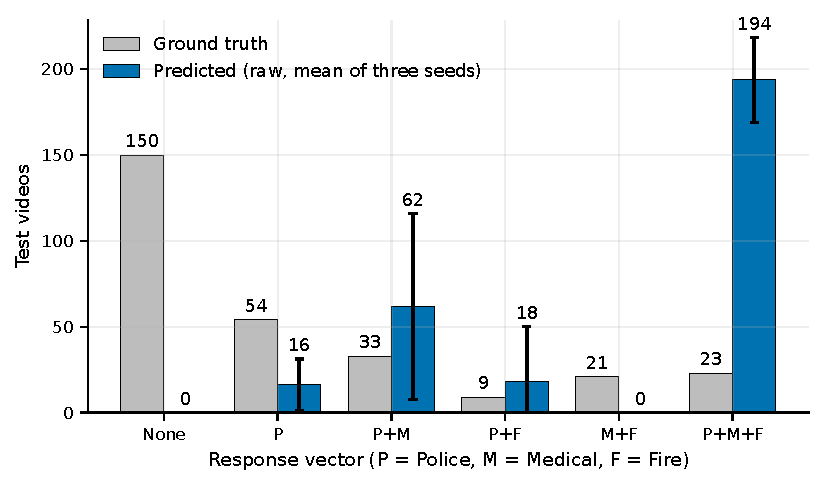
\includegraphics[width=0.88\textwidth]{fig_response_vector_distribution_r20.pdf}
    \caption[Predicted and ground-truth response vectors.]{Raw predicted response vectors (fixed bags, threshold 0.5, no gate; mean and sample SD over three seeds) beside the ground-truth vectors of the 290 test videos.}
    \label{fig:results-joint-dispatch}
\end{figure}

Aggregate metric stability did not imply stable per-video routing. Binary predictions were unanimous across seeds for 95.2\% of test videos, whereas the complete three-bit response vector was unanimous for 51.4\% (Table~\ref{tab:results-unanimity}). Channel-wise unanimity was 100.0\% for Police, 67.6\% for Medical, and 63.4\% for Fire.

\begin{table}[tbp]
    \centering
    \small
    \caption[Cross-seed unanimity of test predictions.]{Share of the 290 fixed-bag test videos on which all three seeds give the same prediction. The complete Police agreement follows from Police being predicted for every video, not from discriminative routing.}
    \label{tab:results-unanimity}
    \begin{tabular}{@{}lc@{}}
        \toprule
        \textbf{Output} & \textbf{Unanimous across seeds (\%)} \\
        \midrule
        Binary decision & 95.2 \\
        Complete response vector & 51.4 \\
        Police & 100.0 \\
        Medical & 67.6 \\
        Fire & 63.4 \\
        \bottomrule
    \end{tabular}
\end{table}

\section{Binary-Gated Routing and Matched Baselines}
\label{sec:results-fixed-routing}
\label{sec:results-fixed-baselines}

Restricting the same raw outputs to the 140 ground-truth anomalous videos increased Macro-F1 to $0.743 \pm 0.013$ (Table~\ref{tab:results-fixed-routing}). This is an oracle-conditioned diagnostic: normal videos and their false-positive opportunities are absent. Applying the learned binary gate over all 290 videos produced Macro-F1 $0.662 \pm 0.022$, reduced Hamming loss from $0.592 \pm 0.033$ to $0.234 \pm 0.016$, and increased exact match from $0.099 \pm 0.020$ to $0.545 \pm 0.009$ on the matched population.

The learned routing views were compared with all-services rules on the same populations. On all 290 videos, always predicting every service obtained Macro-F1 0.437, while the learned raw output obtained $0.478 \pm 0.009$. After using each checkpoint's binary decision, the learned response head obtained $0.662 \pm 0.022$, compared with $0.647 \pm 0.009$ for binary-gated all-services. On the 140 anomalous videos, learned raw routing obtained $0.743 \pm 0.013$, compared with 0.726 for the deterministic all-services rule. Table~\ref{tab:results-fixed-routing} also reports Hamming loss and exact match so that the comparison does not depend on Macro-F1 alone.

\begin{table}[tbp]
    \centering
    \footnotesize
    \caption[Matched fixed-bag routing conditions and baselines.]{Matched response-routing conditions on the test split using immutable 16-instance fixed bags. Learned channels and the learned raw part of the conditions use threshold 0.5; binary-gated rows use each checkpoint's binary argmax. The all-services rows are deterministic single rules and therefore carry no artificial SD, whereas learned and binary-dependent rows show mean $\pm$ sample SD across three checkpoints. The 140-video rows are ground-truth anomaly-conditioned diagnostics; all other rows use all 290 videos. No temporal cases are excluded.}
    \label{tab:results-fixed-routing}
    \begin{tabular}{@{}llccc@{}}
        \toprule
        \textbf{Population} & \textbf{Fixed-bag condition} & \textbf{Macro-F1} & \textbf{Hamming loss} & \textbf{Exact match} \\
        \midrule
        All 290 & Learned raw & $0.478 \pm 0.009$ & $0.592 \pm 0.033$ & $0.099 \pm 0.020$ \\
        All 290 & Learned binary-gated & $0.662 \pm 0.022$ & $0.234 \pm 0.016$ & $0.545 \pm 0.009$ \\
        All 290 & All services & 0.437 & 0.714 & 0.079 \\
        All 290 & Binary-gated all services & $0.647 \pm 0.009$ & $0.254 \pm 0.001$ & $0.534 \pm 0.000$ \\
        \addlinespace
        Anomalous 140 & Learned raw, oracle-conditioned & $0.743 \pm 0.013$ & $0.361 \pm 0.035$ & $0.205 \pm 0.041$ \\
        Anomalous 140 & All services & 0.726 & 0.407 & 0.164 \\
        Anomalous 140 & Binary-gated all services & $0.694 \pm 0.015$ & $0.418 \pm 0.013$ & $0.143 \pm 0.014$ \\
        \bottomrule
    \end{tabular}
\end{table}

The corresponding matched comparisons are small in Macro-F1: the fixed-bag learned gate exceeds binary-gated all-services by 0.015 (95\% video bootstrap interval 0.008 to 0.023), and anomaly-conditional learned routing exceeds all-services by 0.017. Per seed, the gated margin was 0.024, 0.000, and 0.022. For seed 2027, every video that passed the binary gate received all three services, so its gated output coincides with the binary-gated all-services rule on every test video, in the fixed-bag and the dense path alike. The mean margin therefore rests on two of the three checkpoints.

\section{Validation-Only Prototype-Distance Study}
\label{sec:results-ablation}

The $2\times2$ prototype-distance study comprises 12 validation runs: four variants, each trained with the same three seeds used by the official models. Table~\ref{tab:results-ablation} reports the fixed 161-video validation results. The highest mean response Macro-F1 was $0.452 \pm 0.008$ for No input, rather than the Full variant's $0.447 \pm 0.013$.

\begin{table}[tbp]
    \centering
    \small
    \caption[Validation-only prototype-distance study.]{Validation-only prototype-distance results on the immutable 161-video, 16-instance validation bags at response threshold 0.5; binary AUROC is threshold-free. Values are means and sample standard deviations across three training seeds. Checkpoints were selected and reported on this same validation population; none of the 12 runs loaded or evaluated the test split. The table therefore provides descriptive mechanism evidence, not test-performance or general causal evidence.}
    \label{tab:results-ablation}
    \begin{tabularx}{\textwidth}{@{}Xcccc@{}}
        \toprule
        \textbf{Variant} & \textbf{Macro-F1} & \textbf{Binary AUROC} & \textbf{Binary F1} & \textbf{Hamming loss} \\
        \midrule
        Full & $0.4474 \pm 0.0129$ & $0.9444 \pm 0.0002$ & $0.8590 \pm 0.0083$ & $0.5625 \pm 0.0371$ \\
        No input & $0.4520 \pm 0.0082$ & $0.9444 \pm 0.0007$ & $0.8518 \pm 0.0031$ & $0.5493 \pm 0.0303$ \\
        Uniform & $0.4393 \pm 0.0028$ & $0.9431 \pm 0.0002$ & $0.8502 \pm 0.0159$ & $0.5880 \pm 0.0198$ \\
        Neither & $0.4424 \pm 0.0077$ & $0.9415 \pm 0.0022$ & $0.8504 \pm 0.0138$ & $0.5769 \pm 0.0331$ \\
        \bottomrule
    \end{tabularx}
\end{table}

Guided sampling minus uniform sampling changed mean validation Macro-F1 by $+0.008$ when the score was appended and by $+0.010$ without score input. Appending the score changed the mean by $-0.005$ under guided sampling and by $-0.003$ under uniform sampling. With score input, the per-seed differences were $-0.0005$, $+0.019$, and $+0.006$, so guided sampling showed no consistent difference across seeds, and score concatenation did not improve the mean response Macro-F1 in this protocol. Selection on the reported validation set and the absence of test evaluation further preclude a causal conclusion.

\section{Normal-Bag Response-Loss Study (Validation Only)}
\label{sec:results-normal-bag}

The recorded validation history of the three official runs was checked first.
Police was predicted for all 161 validation videos at every logged epoch of
every run, and a minimum-Hamming-loss rule selects the official epoch in all
three runs. Intermediate checkpoints were not saved.

Table~\ref{tab:results-normal-bag} reports both loss variants against their
matched control on the 161-video validation set. \emph{Raw} is the ungated
response output on all videos; \emph{gated} applies each run's own binary
decision to both the learned output and the all-services reference;
\emph{anomalous-only} restricts to the 81 anomalous validation videos. Margins
are taken against the all-services reference of each view (raw 0.4046; gated
0.569--0.583, depending on the run's gate; anomalous-only 0.6520).

\begin{table}[tbp]
    \centering
    \small
    \caption[Normal-bag response-loss study, validation only.]{Normal-bag response-loss study, validation only. The first three columns are Macro-F1 margins over the matched all-services reference. Control is the Full arm of the prototype-distance study, without a normal-bag term; the unweighted variant adds normal bags to a single merged mean; the weighted variant adds them as a separate term ($\lambda=0.3$, fixed before training). Police and Medical precision/recall are on the raw output.}
    \label{tab:results-normal-bag}
    \begin{tabular}{@{}lccccc@{}}
        \toprule
        \textbf{Run} & \textbf{Raw} & \textbf{Gated} & \textbf{Anomalous} & \textbf{Police P / R} & \textbf{Medical P} \\
                     &              &                & \textbf{only}      & \textbf{(raw)}        & \textbf{(raw)} \\
        \midrule
        Control s1337    & +0.031 & +0.019 & +0.023 & 0.484 / 1.000 & 0.232 \\
        Control s2027    & +0.057 & +0.023 & +0.032 & 0.484 / 1.000 & 0.262 \\
        Control s3407    & +0.040 & +0.007 & +0.010 & 0.484 / 1.000 & 0.213 \\
        Unweighted s1337 & +0.184 & +0.007 & +0.015 & 0.735 / 0.962 & 0.390 \\
        Unweighted s2027 & +0.205 & +0.024 & +0.029 & 0.755 / 0.949 & 0.392 \\
        Unweighted s3407 & +0.189 & +0.017 & +0.025 & 0.735 / 0.962 & 0.380 \\
        Weighted s1337   & +0.164 & +0.019 & +0.032 & 0.685 / 0.974 & 0.356 \\
        Weighted s2027   & +0.177 & +0.020 & +0.032 & 0.681 / 0.987 & 0.372 \\
        Weighted s3407   & +0.169 & +0.017 & +0.034 & 0.658 / 0.987 & 0.372 \\
        \bottomrule
    \end{tabular}
\end{table}

Under the unweighted variant, raw Police precision rose from 0.484 (the
control, like the official checkpoints, predicted Police for all 161
validation videos) to 0.735--0.755, with recall falling from 1.000 to
0.949--0.962; false positives on the 80 normal validation videos fell from 80
to 21--24. Once both arms are gated identically, or restricted to the
anomalous videos, the variant's margin is indistinguishable within the
seed-to-seed spread from the control's (mean gated margin +0.016 in both
arms; mean anomalous-only margin +0.023 versus +0.022). Police still activates
on all three Explosion validation videos in every variant, the one category
the mapping assigns Police $=0$.

Against the unweighted variant, the weighted variant (Section~\ref{sec:normal-bag-study}) changed the margins as follows: the anomalous-only margin
rose by 0.0099, about 1.4 times the unweighted variant's seed standard
deviation of 0.0070, while the gated margin moved by 0.0026. Medical precision
fell by 0.021, Fire precision by 0.015, and Police precision by 0.067, about
six times the unweighted variant's spread; mean raw Macro-F1 was 0.574 versus
0.597. No other weight was tried.

\section{Dense Indexed-System and Temporal-Grounding Results}
\label{sec:results-dense-temporal}

\subsection{Dense Indexed Binary and Routing Results}

Table~\ref{tab:results-dense-routing} reports evaluation of the same three checkpoints on all 69,090 indexed test clips. Dense binary AUROC was $0.942 \pm 0.001$ and positive-class F1 was $0.874 \pm 0.010$. Raw, binary-gated, and anomaly-conditional response Macro-F1 values were $0.473 \pm 0.010$, $0.660 \pm 0.020$, and $0.740 \pm 0.012$, respectively. These values remain distinct from the fixed-bag results because every video's input bag changed.

\begin{table}[tbp]
    \centering
    \small
    \caption[Dense indexed binary and response results.]{Dense indexed-system results on the test split (variable-length bags, all 69,090 clips of the 290 videos). Binary AUROC is threshold-free; the other binary metrics use argmax; response metrics use threshold 0.5, with gating stated per block. The SD is the sample SD over the three Stage-2 seeds. The 140-video rows are oracle anomaly-conditioned and include the five videos with annotation-boundary conflicts.}
    \label{tab:results-dense-routing}
    \begin{tabular}{@{}lcccc@{}}
        \toprule
        \textbf{View and metric} & \textbf{Seed 1337} & \textbf{Seed 2027} & \textbf{Seed 3407} & \textbf{Mean $\pm$ sample SD} \\
        \midrule
        \multicolumn{5}{@{}l}{\emph{Binary, all 290 videos}} \\
        Accuracy & 0.883 & 0.872 & 0.886 & $0.880 \pm 0.007$ \\
        AUROC & 0.940 & 0.942 & 0.943 & $0.942 \pm 0.001$ \\
        Positive-class precision & 0.890 & 0.899 & 0.885 & $0.891 \pm 0.007$ \\
        Positive-class recall & 0.864 & 0.829 & 0.879 & $0.857 \pm 0.026$ \\
        Positive-class F1 & 0.877 & 0.862 & 0.882 & $0.874 \pm 0.010$ \\
        \addlinespace
        \multicolumn{5}{@{}l}{\emph{Response raw, all 290 videos}} \\
        Macro-F1 & 0.483 & 0.464 & 0.470 & $0.473 \pm 0.010$ \\
        Hamming loss & 0.571 & 0.639 & 0.609 & $0.607 \pm 0.034$ \\
        Exact match & 0.114 & 0.083 & 0.090 & $0.095 \pm 0.016$ \\
        \addlinespace
        \multicolumn{5}{@{}l}{\emph{Response binary-gated, all 290 videos}} \\
        Macro-F1 & 0.671 & 0.638 & 0.672 & $0.660 \pm 0.020$ \\
        Hamming loss & 0.225 & 0.253 & 0.230 & $0.236 \pm 0.015$ \\
        Exact match & 0.552 & 0.534 & 0.545 & $0.544 \pm 0.009$ \\
        \addlinespace
        \multicolumn{5}{@{}l}{\emph{Response raw, 140 anomalous videos}} \\
        Macro-F1 & 0.751 & 0.727 & 0.743 & $0.740 \pm 0.012$ \\
        Hamming loss & 0.340 & 0.402 & 0.362 & $0.368 \pm 0.031$ \\
        Exact match & 0.236 & 0.171 & 0.186 & $0.198 \pm 0.034$ \\
        \bottomrule
    \end{tabular}
\end{table}

The dense all-services baseline remained at Macro-F1 0.437. Dense binary-gated all-services reached $0.646 \pm 0.008$, compared with $0.660 \pm 0.020$ for learned binary-gated routing on all 290 videos. On the conditional 140-video population, all services reached 0.726, binary-gated all services reached $0.692 \pm 0.012$, and learned raw routing reached $0.740 \pm 0.012$. Figure~\ref{fig:results-routing-comparison} places these dense results beside their fixed-bag counterparts under matched populations.

\begin{figure}[tbp]
    \centering
    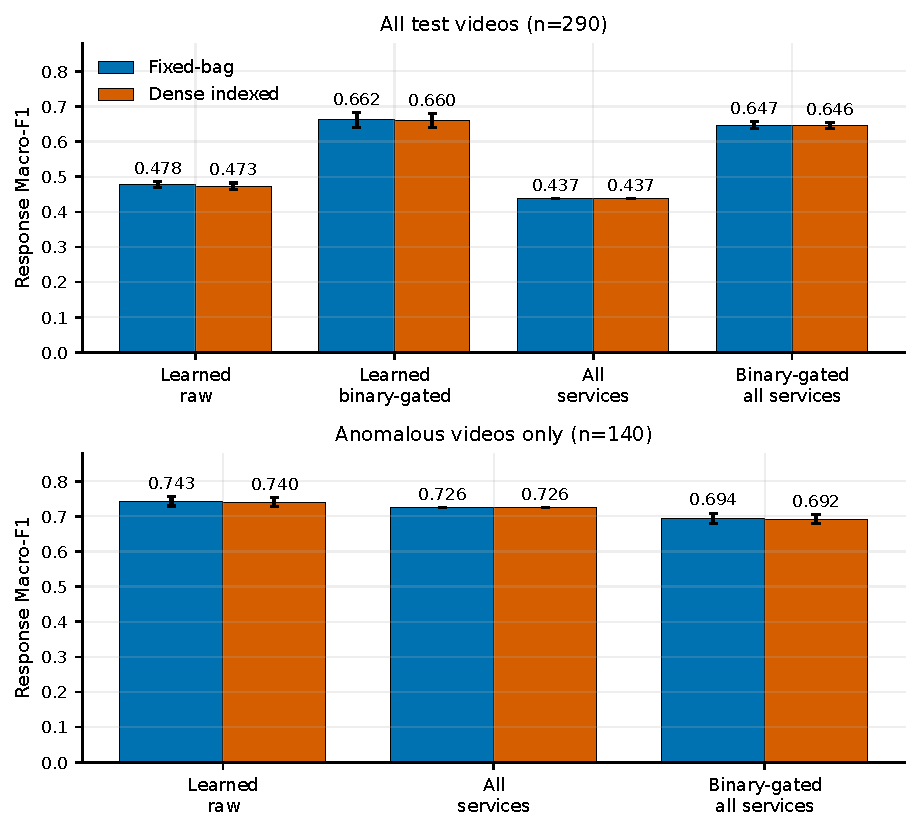
\includegraphics[width=\textwidth]{fig_routing_comparison_r20.pdf}
    \caption[Matched fixed-bag and dense routing comparisons.]{Response Macro-F1 of learned outputs and all-services rules on the fixed-bag and dense indexed inputs (threshold 0.5; gated conditions use the binary argmax). Top: all 290 test videos. Bottom: the 140 anomalous videos, an oracle-conditioned diagnostic. Error bars: sample SD over three seeds; all-services is one deterministic rule.}
    \label{fig:results-routing-comparison}
\end{figure}

\subsection{Dense Coverage}

The realized dense store covered 1,110,064 of 1,111,808 source frames, or 99.843\% frame-weighted coverage. Its mean per-video coverage was 99.540\%, the median was 99.758\%, and the minimum was 92.903\%. All annotated frames in the 135 temporally eligible anomaly videos were covered. Under the same source-frame geometry, sparse-store and fixed-bag frame-weighted coverage were 50.896\% and 12.062\%, respectively. These quantities describe which frames could be observed by each input construction; they are not performance metrics.

\subsection{Primary Temporal Grounding}

On the 135 source-bounded anomalous videos, mean temporal AP was $0.327 \pm 0.014$ and top-clip hit rate was $0.291 \pm 0.004$. At the primary interval threshold of 0.5, fixed before the dense evaluation, mean IoU was $0.186 \pm 0.017$ and $0.193 \pm 0.053$ of eligible videos had exactly zero IoU. The fractions with IoU of at least 0.1, 0.3, 0.5, and 0.7 were $0.558 \pm 0.026$, $0.215 \pm 0.032$, $0.074 \pm 0.007$, and $0.022 \pm 0.000$, respectively.

The separate binary-gated display rule at temporal threshold 0.65 produced mean IoU $0.128 \pm 0.014$ and zero-IoU frequency $0.425 \pm 0.045$. On the 150 normal videos, the ungated primary rule produced at least one interval for every video and assigned $0.379 \pm 0.056$ of source frames to predicted support. The binary-gated display rule produced at least one interval for $0.098 \pm 0.010$ of normal videos and assigned $0.026 \pm 0.006$ of their source frames to predicted support.

Temporal AP varied across the anomaly categories, whose test supports range from 2 to 23 videos; the per-category values are shown in Appendix Figure~\ref{fig:results-temporal-category}.

\subsection{Frozen Temporal References}

Table~\ref{tab:results-temporal-baselines} compares the learned attention with the four checkpoint-independent references. The whole-video reference scores every frame equally, so its AP equals the mean event prevalence of 0.191 and marks the chance level of AP. The learned model's temporal AP exceeded each reference; its mean gap to the whole-video reference was 0.136 (95\% video bootstrap interval 0.110 to 0.164). Its primary fixed-rule IoU was below the whole-video reference by 0.005 and above the random-clips and prototype-distance references. The uniform-clips rule had AP 0.192 but produced an empty interval after constant-score normalization for every eligible video, giving IoU zero and a zero-IoU frequency of one. The whole-video reference had zero zero-IoU cases because it always predicts the complete source duration.

\begin{table}[tbp]
    \centering
    \small
    \caption[Dense temporal model and frozen references.]{Temporal grounding on the 135 source-bounded anomalous test videos using the 69,090-clip dense indexed input; five boundary-conflict videos are excluded only here. AP and top-clip hit are threshold-free. Learned fixed-rule IoU uses the 0.5 temporal threshold and is summarized as mean $\pm$ sample SD across three checkpoints. Each reference is one frozen checkpoint-independent replicate under the same geometry and receives no fabricated SD; uniform constant scores yield empty predicted intervals by rule. No response threshold or binary gate is applied.}
    \label{tab:results-temporal-baselines}
    \begin{tabular}{@{}lcccc@{}}
        \toprule
        \textbf{Temporal method} & \textbf{AP} & \textbf{Top-clip} & \textbf{Fixed-rule} & \textbf{Zero-IoU} \\
                                  &              & \textbf{hit}      & \textbf{IoU}        & \textbf{frequency} \\
        \midrule
        Learned attention & $0.327 \pm 0.014$ & $0.291 \pm 0.004$ & $0.186 \pm 0.017$ & $0.193 \pm 0.053$ \\
        Whole video & 0.191 & --- & 0.191 & 0.000 \\
        Uniform clips & 0.192 & 0.015 & 0.000 & 1.000 \\
        Seeded random clips & 0.246 & 0.200 & 0.161 & 0.067 \\
        Prototype distance & 0.277 & 0.244 & 0.110 & 0.363 \\
        \bottomrule
    \end{tabular}
\end{table}

\section{Qualitative Success and Failure Cases}
\label{sec:results-qualitative}

Figure~\ref{fig:results-qualitative} shows four seed-1337 dense records chosen by fixed rules rather than by inspection. The \emph{best case} is the eligible anomalous video with the highest primary IoU among those with a correct binary decision and an exactly correct gated response vector. The \emph{median case} has the median primary IoU of the 135 eligible videos. The \emph{confident misplaced detection} is the zero-IoU video with the highest binary score, and the \emph{false alarm} is the normal video with the highest binary score. Ties are broken by video identity.

\begin{figure}[tbp]
    \centering
    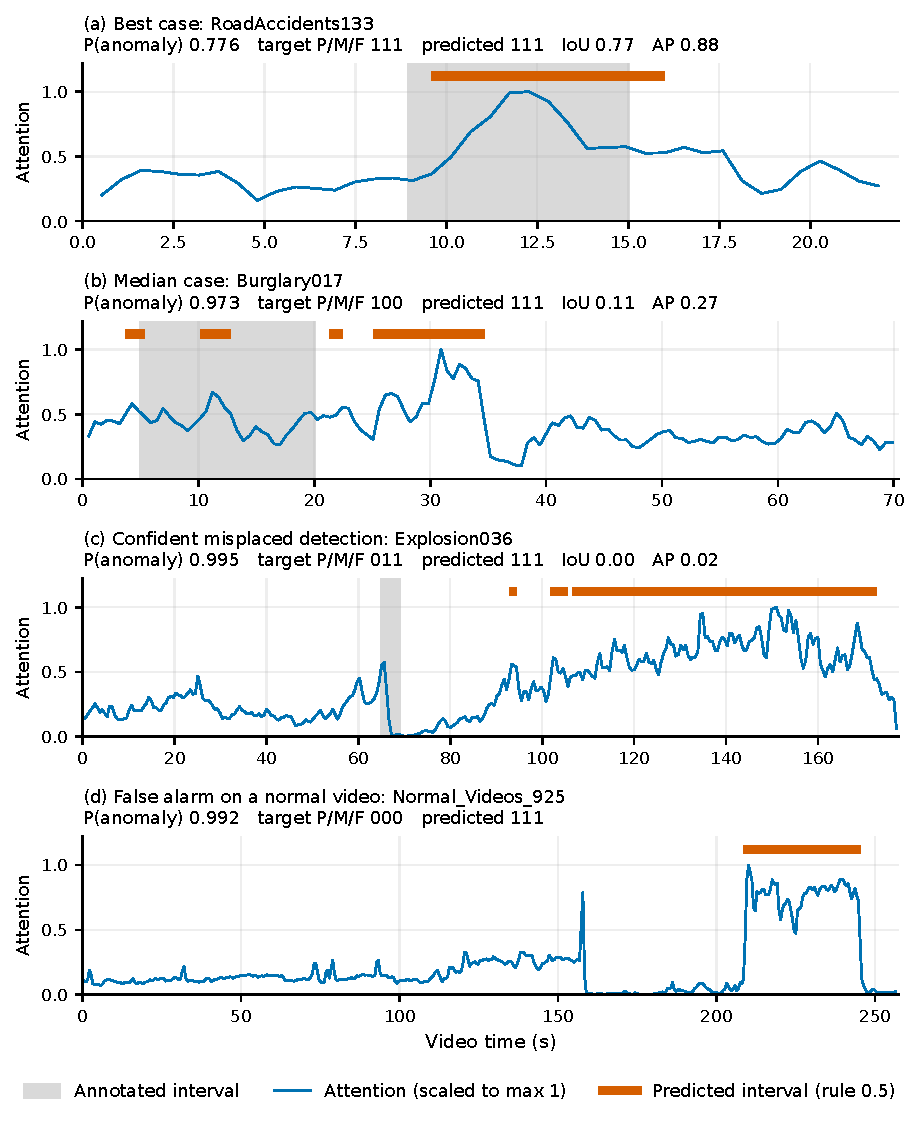
\includegraphics[width=\textwidth]{fig_qualitative_cases_r20.pdf}
    \caption[Qualitative success and failure cases.]{Four seed-1337 dense test records selected by the rules in Section~\ref{sec:results-qualitative}. Each panel shows the attention per clip (scaled to its maximum), the annotated interval, and the interval predicted by the primary rule. Target and predicted response vectors are given as Police/Medical/Fire bits. The videos are from UCF-Crime \cite{sultani2018real}.}
    \label{fig:results-qualitative}
\end{figure}

In the best case, \code{RoadAccidents133}, attention peaks at 12.3\,s inside the annotated interval of 9.0--15.0\,s, and the predicted interval of 9.6--16.0\,s gives IoU 0.77 and AP 0.88. Its correct response vector contains all three services, which is the vector the all-services rule would also produce. In the median case, \code{Burglary017}, the annotated interval is 5.0--20.0\,s, but attention peaks at 30.9\,s; the four predicted intervals overlap the event only in part, giving IoU 0.11, and the response vector adds Medical and Fire to the target Police. In \code{Explosion036}, the binary score is 0.995, but the annotated event lasts from 65.0 to 69.0\,s, while all predicted intervals lie between 92.8 and 172.8\,s; Police is predicted although the mapping assigns no Police to Explosion. The normal video \code{Normal\_Videos\_925} receives a binary score of 0.992, all three services, and a predicted interval of 208.5--245.3\,s.

\section{Offline CAD-Style Example}
\label{sec:results-cad-example}

Figure~\ref{fig:results-cad-example} presents the CAD-style record of a fixed example: the lexicographically first eligible anomalous seed-1337 output that triggered an alert, \code{Abuse/Abuse028\_x264.mp4}. Temporally, this example is a failure case. The dense bag contains 87 clips and covers 1,408 of 1,412 source frames. The target response is Police and Medical. The binary anomaly score is 0.897 and the binary decision is Anomaly. At the scientific response threshold of 0.5, the response vector is Police, Medical, and Fire. At the separate display thresholds $[0.65,0.60,0.65]$, the CAD-style record retains Police and Medical and assigns \code{P1-MEDICAL}.

The source-bounded annotation is frames $[164,240)$, while the primary 0.5 temporal rule predicts $[0,176)$ and $[320,352)$, giving IoU 0.044. The display rule predicts $[0,160)$ and therefore has IoU zero. Its displayed window is 0.00--5.33 seconds, whereas the annotated interval begins at 5.47 seconds: the alert is raised from the first second of the video, before the annotated event has begun. The stored \code{alert\_latency\_sec} is 0.00 because it records the displayed source-video timestamp, not computation time or delay from event onset.

\begin{figure}[tbp]
    \centering
    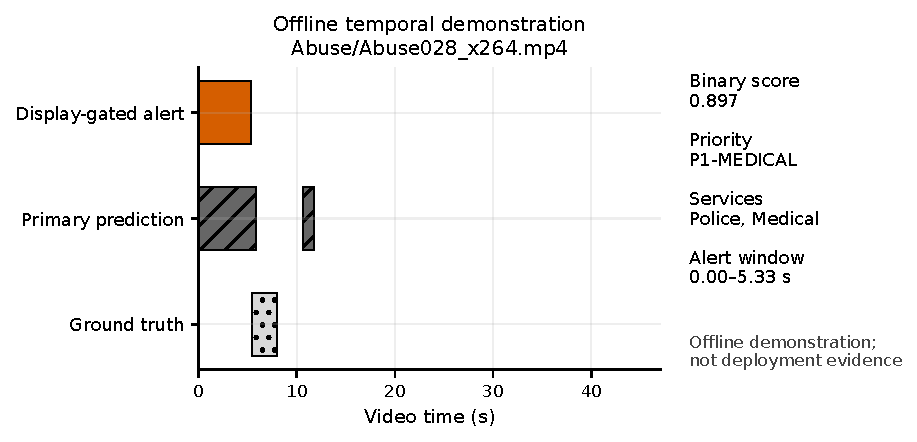
\includegraphics[width=\textwidth]{fig_temporal_cad_example_r20.pdf}
    \caption[Qualitative offline CAD-style record.]{Offline seed-1337 example for \code{Abuse/Abuse028\_x264.mp4}, selected by a deterministic lexical rule rather than performance; temporally a failure case (primary IoU 0.044). The dense input has 87 clips; the primary temporal rule uses threshold 0.5, while the displayed interval uses threshold 0.65 and the binary gate. Scientific response decisions use threshold 0.5; the displayed Police/Medical/Fire thresholds are $[0.65,0.60,0.65]$. This is one saved test record with no replicate uncertainty. It demonstrates deterministic rendering of model output, not live latency, external CAD integration, reliability, or safety.}
    \label{fig:results-cad-example}
\end{figure}

Figure~\ref{fig:results-cad-frame} shows the same record as an operator-facing overlay rendered on the source frame, rather than the schematic timeline above.

\begin{figure}[tbp]
    \centering
    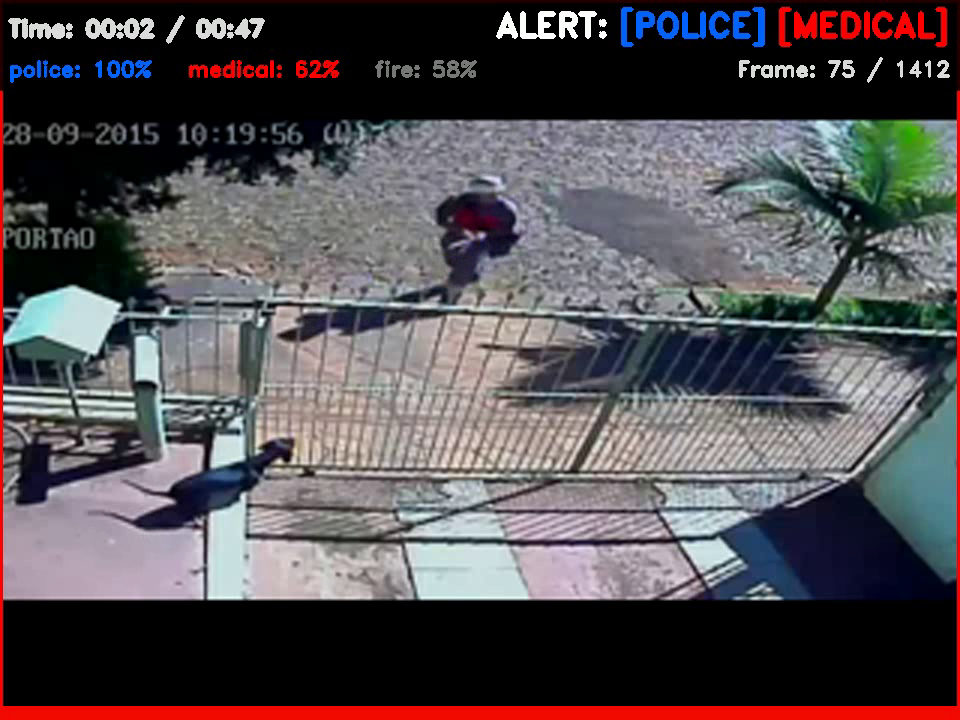
\includegraphics[width=0.8\textwidth]{fig_cad_frame_example.png}
    \caption[Rendered CAD-style overlay, source frame.]{Source-video frame at time 2.50\,s for the same \code{Abuse/Abuse028\_x264.mp4} seed-1337 example, inside the displayed alert window $[0.00,5.33]$\,s, rendered by the offline overlay tool (checkpoint \code{dispatch\_repro\_s1337}) rather than the fixed-bag or dense evaluation pipelines. Displayed confidences are rounded (police 100\%, medical 62\%, fire 58\%) from the same values as Figure~\ref{fig:results-cad-example}. This is UCF-Crime surveillance footage of a real scene \cite{sultani2018real}, shown once as a rendering example; it is not a live capture and is not deployment or safety evidence.}
    \label{fig:results-cad-frame}
\end{figure}

Figure~\ref{fig:results-cad-json} shows the stored alert record for the same example. It holds one alert window given by start and end frame, the dispatched services, the priority, and the per-channel confidences. It does not hold per-frame labels or an anomaly category.

\begin{figure}[tbp]
    \centering
    \begin{minipage}{0.75\textwidth}
\begin{lstlisting}[basicstyle=\ttfamily\footnotesize]
{
  "timestamp": "2026-09-27T10:13:59.510023",
  "source_video": "data/ucf_crime/raw/Abuse/
                   Abuse028_x264.mp4",
  "alert_triggered": true,
  "dispatch": ["police", "medical"],
  "priority": "P1-MEDICAL",
  "anomaly_window": {
    "start_frame": 0,
    "end_frame": 159,
    "start_sec": 0.0,
    "end_sec": 5.33
  },
  "confidence": {
    "police": 0.9994,
    "medical": 0.6235,
    "fire": 0.5785
  },
  "alert_latency_sec": 0.0
}
\end{lstlisting}
    \end{minipage}
    \caption[Stored alert record for the CAD-style example.]{Alert record stored for the same \code{Abuse/Abuse028\_x264.mp4} seed-1337 example (checkpoint \code{dispatch\_repro\_s1337}), with the \code{dispatch} list written on one line and the source path wrapped for width; all values are as stored. The window is stored as inclusive frames 0--159, which is the half-open interval $[0,160)$ used in the text. The record names the dispatched services, not an anomaly category.}
    \label{fig:results-cad-json}
\end{figure}

\section{Factual Summary}
\label{sec:results-summary}

Binary detection was consistent across the three checkpoints and both input paths, with an AUROC near 0.94 and a positive-class F1 near 0.87. The ungated response head had near-complete recall but low precision, and it predicted Police for every video. Binary gating improved all response metrics, yet the learned gated Macro-F1 stayed only slightly above the gated all-services rule. The two validation-only studies showed no consistent effect of guided sampling, of appending the distance, or of adding normal bags beyond removing the universal Police output. On the dense protocol, which covers 99.843\% of the test-video frames, temporal attention reached an AP of 0.327 and an IoU of 0.186, with 19.3\% of eligible videos at zero IoU. The four qualitative cases show one well-localized event and three confident decisions with misplaced intervals or a false alarm.

% !TeX root = ../thesis.tex
\chapter{Discussion}
\label{chap:discussion}

This chapter first answers the research questions, then interprets why the
three outputs behave so differently, relates the findings to prior work, and
draws implications before turning to limitations, ethics, and future work.
Numbers are repeated only where an argument depends on them; the complete values
are in Chapter~\ref{chap:results}.

\section{Answers to the Research Questions}
\label{sec:discussion-rq-answers}

\subsection{RQ1: Video-Level Binary Anomaly Detection}
\label{sec:discussion-rq1}

Video-level binary detection is the solid result of the thesis. All three
checkpoints reached an AUROC of about 0.94 on both the fixed-bag and the dense
indexed input (Tables~\ref{tab:results-fixed-binary}
and~\ref{tab:results-dense-routing}), and their binary decisions agreed on
95.2\% of the test videos. Resampling the test videos moves the fixed-bag
AUROC between about 0.91 and 0.97, which is wider than the spread between seeds.
This holds for the pipeline as executed, with one adapted feature store and one prototype memory. No experiment isolates the contribution of LoRA, the prototypes, or MIL (Section~\ref{sec:discussion-binary}).

\subsection{RQ2: Historical and Response-Label Error Profiles}
\label{sec:discussion-rq2}

The historical 14-class outputs concentrated their predictions on Normal and
recognized the anomaly categories poorly (Table~\ref{tab:results-historical}).
The three-channel response formulation fails differently. Its raw output has
near-complete recall but low precision, activates Police for every video, and
never predicts the empty or the Medical-and-Fire vector
(Table~\ref{tab:results-fixed-raw}, Figure~\ref{fig:results-joint-dispatch}).
The two tasks are not a before-and-after comparison. Adding normal bags to the
response loss removed the universal Police output on validation, but did not
improve service selection beyond the seed spread of the control
(Table~\ref{tab:results-normal-bag}).

\subsection{RQ3: Stage-2 Stability and Matched Binary Gating}
\label{sec:discussion-rq3}

Binary decisions are stable across the three Stage-2 seeds; complete response
vectors are not, with unanimity for only half of the test videos
(Table~\ref{tab:results-unanimity}). Binary gating changes the matched error
profile substantially (Table~\ref{tab:results-fixed-routing}), but almost all
of that change also occurs when every service is predicted after the same gate.
The learned head adds 0.015 in Macro-F1 over that rule. The margin is positive
under video resampling, but it comes from two of the three seeds: for seed 2027
the learned gated output is identical to the rule.

\subsection{RQ4: Dense Indexed Temporal Alignment}
\label{sec:discussion-rq4}

Attention aligns with annotated intervals measurably but weakly. Its temporal
AP exceeds all four frozen references, with a gap to the whole-video chance
level that stays clearly positive under video resampling
(Table~\ref{tab:results-temporal-baselines}). Its interval overlap, however,
stays at the level of predicting the whole video, and one eligible video in five
receives an interval that misses the event entirely. Attention is therefore a
weak temporal ranking signal, not an event-boundary estimator.

\section{Interpretation}
\label{sec:discussion-evidence}

\subsection{Why the Response Head Defaults to Police}
\label{sec:discussion-police}

The universal Police output follows from the target design and the loss. In
the project mapping, Police is positive for every anomaly category except
Explosion (Table~\ref{tab:response-map}); 703 of the 729 anomalous training bags
(96\%) carry a Police label. The response loss is evaluated on anomalous bags
only (Section~\ref{sec:optimization}), so the head is never trained toward an
all-zero vector. An output that always activates Police therefore loses little,
and this is what the trained heads do: Police precision equals $119/290$ in every
seed, the value obtained by assigning Police to every test video. Because the
official runs predicted Police for every validation video at every logged epoch
(Section~\ref{sec:results-normal-bag}), no checkpoint-selection rule could have
avoided it.

Medical and Fire are over-predicted as well, but not as a copy of their prior.
Among anomalous training bags, 39.8\% carry Medical and 24.3\% carry Fire; the
heads predicted them for 88.0\% and 73.1\% of the test videos. Their precision
lies above the test prevalence, by about a third for Fire, but far from what
selective routing would require. Two further properties of the objective push
in the same direction and were not varied: the asymmetric loss down-weights
negative targets strongly ($\gamma_-=6$, \cite{ridnik2021asymmetric}), and the
response threshold of 0.5 was never tuned. Either can raise the share of
positive decisions independently of the features.

\subsection{What the Normal-Bag Study Does and Does Not Show}

Adding normal bags to the response loss removes the symptom it targets: raw
Police precision on validation rises, and the response head no longer
predicts Police for most normal videos. The raw margins in Table~\ref{tab:results-normal-bag}
therefore mostly show that the response head now also separates normal from
anomalous videos, which the binary head already does. Once both arms are gated
identically, or restricted to the anomalous videos, the variant does not differ
from the control beyond the seed spread, and Police still fires on every
Explosion video. The weighted variant makes the simplest explanation, that the
merged mean diluted the anomalous signal, unlikely. Leaving normal bags out of the
response loss thus explains the universal Police output, but not the weak
service selection.

A plausible further cause lies upstream. Each response vector is a fixed
function of the anomaly category, so a head can only select services as well as
the features separate the categories. The encoder,
\code{MCG-NJU/videomae-base}, is the self-supervised pre-trained VideoMAE
checkpoint \cite{tong2022videomae}, which is intended to be fine-tuned on a
downstream task, and its mean-pooled clip features were adapted here only once,
with inherited clip labels. Whether these features separate the 13 categories
was not tested, so this is only a hypothesis about this checkpoint and adaptation.

\subsection{Why the Binary Gate Supplies Most of the Value}

Binary gating suppresses all response positives after a Normal decision. Since
the raw head predicts at least Police for every normal video, this removes most
of its false positives, and the large changes in Macro-F1, Hamming loss, and
exact match follow. The binary-gated all-services rule receives the same
benefit without learning anything about services, which is why it is the
relevant reference. The remaining learned margin is small, rests on two of three
seeds, and should be read against a second source of variation: in the
validation studies, changing only how the training bags were drawn moved
validation Macro-F1 by up to 0.033 for the same seed
(Section~\ref{sec:method-limits}). A margin of this size is therefore a description
of these three checkpoints on these 290 videos, not an established property of
the method. The low unanimity of complete response vectors points the same way:
small aggregate standard deviations do not imply that a video receives the same
services from each checkpoint.

\subsection{What the Binary Detector May Rely On}
\label{sec:discussion-binary}

The binary result is consistent with event-related evidence, but an alternative
cannot be excluded. The fixed bags observe about 12\% of the source frames, the
dense input almost all of them, and the AUROC is the same. One reading is that
16 clips already carry the usable evidence. Another is that the decision relies
on properties shared by the whole video, such as scene, camera, resolution, or
compression, which differ between UCF-Crime's normal and anomalous recordings.
Abdulaziz and Bondarev report that, on normal footage alone, every model they
examined separates UCF-Crime videos by such recording properties
\cite{abdulaziz2026auditing}. The weak temporal grounding is compatible with
both readings. The selection history adds a further point: the seed-2027
checkpoint is its epoch-0 model and reaches the same AUROC as the others, so the
binary separation is largely available after one epoch of Stage-2 training on
the fixed features and prototype distance. Neither shortcut probes nor a
matched frozen-feature or mean-pooling baseline were run, so the binary result
cannot be attributed to any single component.

\subsection{Prototype Distance}

In the validation-only study, guided sampling showed no consistent difference
across seeds and appending the distance did not raise mean Macro-F1. One
possible reason is the input scale: the distance is a single value between 0
and 4 appended to a 768-dimensional unnormalized embedding
(Equation~\ref{eq:augmented-instance}), so its influence on the attention scorer
may be small. The study uses one validation split that also selected the checkpoints, so it neither supports nor rules out a benefit on test data.

\subsection{Why Temporal AP and IoU Disagree}
\label{sec:discussion-temporal}

AP rewards the ranking of frames, whereas IoU judges the single interval that
the fixed rule extracts from that ranking. The rule normalizes the smoothed
attention to the range of each video, so it always marks the upper part of that
range, whatever the absolute attention level. It produced an interval for every
normal test video, and on anomalous videos it can mark a broad or displaced
region even when annotated frames rank high. A broad interval approaches the
whole-video reference, which is consistent with the learned IoU lying at that
reference's level. The AP gain, in turn, is measured against a chance level
that equals the event prevalence; events covering most of a video raise the AP
of every method.

The qualitative cases in Figure~\ref{fig:results-qualitative} show both failure
types. In \code{Burglary017} and \code{Explosion036}, attention peaks after the
annotated event, and in the false alarm a confident binary score coincides with
a sharp attention block in a normal video. Two properties of the setup may
contribute. The model was trained on 16-instance bags but is applied to dense
bags of about 238 clips, and softmax attention changes its scale with bag
length; the near-complete dense coverage makes input sparsity an unlikely
explanation, but not this length shift. In addition, attention was trained only
to pool evidence for the video label, not to localize, and standard attention
weights need not explain a model's decision \cite{jain2019attention}. No alternative interval rule or bag length was evaluated, so both remain explanations. The category-level AP values
(Appendix~\ref{app:temporal-category}) rest on two to 23 videos per category and
do not support a ranking of categories.

\subsection{Historical Task Reformulation}
\label{sec:discussion-historical}

The historical 14-class outputs motivated the response formulation, but they
are not an ablation. Their two runs differ in features, prototype inputs,
training settings, and provenance, so their difference is not an effect of
LoRA. The three-channel formulation was chosen because it can represent
overlapping services, which one exclusive label cannot. It did not remove the
failure: predominant Normal prediction gave way to high-recall over-prediction,
and the two tasks share no metric that would make a numerical comparison
meaningful.

\section{Relation to Prior Work}
\label{sec:discussion-prior-work}

The methods in Table~\ref{tab:related-comparison} report detection as one
frame-level AUC per method. This thesis measures something different and cannot
place itself in that ranking: its AUROC is video-level, and its temporal
evaluation is per video. Two observations nevertheless connect the findings to
the literature. First, Abdulaziz and Bondarev argue that pooled frame-level AUC
mixes localization with differences between recording sources and cannot
resolve small margins on the UCF-Crime test split \cite{abdulaziz2026auditing}.
The present results point to the same two issues from a different angle: a
strong video-level score coexists with weak per-video localization, and the
headline margins of this thesis are small relative to test-sampling and
training variation. Second, none of the compared methods has a response output,
so none reports a matched rule for one. The comparison with binary-gated all-services shows
why such a rule matters: without it, the gated Macro-F1 of 0.662 would suggest
a response capability that the head largely does not have. Recent
vision-language methods such as VadCLIP and Holmes-VAD name or describe
anomalies \cite{wu2024vadclip,zhang2024holmes}; whether their outputs select
services better than a matched rule is an open question that the same kind of
reference could answer.

\section{Implications}
\label{sec:discussion-implications}

For weakly supervised video anomaly detection, the results suggest three
reporting practices: compare each learned output with a trivial rule on the same
population and after the same gate; evaluate temporal evidence per video
against a whole-video reference, whose AP equals the event prevalence; and
report training variation over seeds separately from test-sampling uncertainty
over videos. Each is cheap, and each changed the reading of a result in this
thesis.

For response-oriented work, the main implication concerns the targets. A
deterministic category-to-service lookup makes Police the default of the label
space, and a model trained on it learns that default. Response targets that can
reward selective behavior need independently annotated or observed service
needs. The base rate matters as well. On the dense input, about one normal
video in ten received a binary false positive, and the binary recall was about
0.86. If, for illustration, one recording in a hundred contained an event, a
thousand recordings would yield about nine true alerts and about 97 false ones,
roughly eleven false alerts for each true alert. The test split, with almost
half of its videos anomalous, hides this ratio.

\section{Limitations}
\label{sec:discussion-limitations}

\subsection{Evaluation History and Statistical Scope}

The fixed test outcomes had been inspected before this thesis was written.
Development-stage runs that predate the frozen protocol were also evaluated on
the test split; they are not reported, while the official protocol is reported
in full. Section~\ref{sec:method-limits} separates design constants recorded
before the first test evaluation from inherited ones. This history raises the
risk that earlier choices were indirectly informed by test behavior, and a
credible next evaluation needs an external test set or a nested design.

Two kinds of uncertainty are reported, and both are partial. The sample
standard deviations describe three Stage-2 runs over the same adapter, features,
prototypes, and evaluation artifacts, not whole-pipeline variation. The bootstrap
intervals describe the sampling of the 290 test videos, not training variance or
variation across sites. Neither licenses a population-level reliability claim.
The validation curves stay close to the all-services reference, so checkpoint
selection operates near a noise floor: the selected epochs differ widely,
including epoch 0 for seed 2027, and differences between seeds are not read as
differences between trained models. The Full arm of the prototype-distance study
does not reproduce the official checkpoints because its training bags were drawn
differently (Section~\ref{sec:method-limits}), which bounds how far small
validation margins can be interpreted.

No matched experiment isolates a component: there is no Stage-2 run on
non-adapted features, no mean-pooling baseline, no category-separability probe,
and no alternative encoder. The thesis therefore makes no claim about the
contribution of LoRA, the prototype memory, or MIL. The historical 14-class
outputs are saved outputs, not controlled experiments, and the two validation
studies use the same split for selection and reporting.

\subsection{Dataset, Supervision, and Target Validity}

All quantitative evidence comes from UCF-Crime, with its cameras, categories,
recording conditions, and event prevalence. There is no external dataset, new
site, or cross-camera holdout, so no generalization claim is made. Supervision is
weak at two levels: sampled clips inherit a video category during adaptation,
and one video-level target supervises each Stage-2 bag. Both can entangle scene
and camera cues with the event signal.

The temporal annotations are read as one-based and inclusive, following the
referenced evaluation code, but the convention of the released coordinates was
not independently established. Five annotations end beyond the decoded source
length; they were left unmodified and excluded from temporal metrics only.

Most importantly, Police, Medical, and Fire are not observed service decisions.
They are deterministic project labels derived from UCF-Crime categories; no
dispatcher or other domain expert validated the mapping, and no attendance or
outcome data were available. Metrics against these vectors measure agreement
with the project transformation, not the correctness or necessity of a real
response.

\subsection{Decision Quality, Calibration, and Grounding}

Routing uses fixed thresholds of 0.5 and is not calibrated. There is no
abstention or referral option, no cost matrix, and no operational baseline such
as dispatcher decisions. Temporal grounding relies on one shared attention
mechanism and a fixed rule; attention was not trained with interval labels, no
alternative grounding method or bag length was compared, and there is no spatial
grounding of where in a frame an event occurs. Apart from the timing of one local dense-extraction batch
and the number of trainable adapter parameters, computational cost was not
measured, so the thesis makes no efficiency claim.

\subsection{Representation and Reproducibility Boundaries}

The retained Transformers 5.12.0 loader, which leaves 36 newly represented
biases at zero (Section~\ref{sec:videomae-lora}; Appendix~\ref{app:repro-limits}),
is a compatibility decision, not proof that every pretrained parameter was
reconstructed faithfully, and the persisted \code{float16} prototypes
approximate unavailable \code{float32} centers. The fixed identities and
verification scripts make the named evidence auditable, and a fresh clone with
the local evidence bundle passes the evidence verifiers. Raw videos, checkpoints,
and feature stores remain local and Git-ignored, however, no external archive
exists yet, and the sparse subset used a Python hash seed that was not recorded.
Reproduction claims therefore remain conditional on the preserved local
artifacts and their hashes.

\subsection{Operational Scope}

The evaluated path is offline: it reads stored clips or embeddings, loads fixed
checkpoints, and writes saved CAD-style records. It has not been tested with live
streams, multiple cameras, failures, or operational load, and there is no
external CAD integration, operator study, security analysis, privacy control,
fairness evaluation, or prospective safety evaluation.

\section{Ethical Implications and Human Oversight}
\label{sec:discussion-ethics}

The points below are requirements derived from the measured failure modes, not
capabilities of the prototype. Surveillance models can inherit harm at every
stage of the machine-learning lifecycle \cite{suresh2021framework}. This project
has no demographic attributes or subgroup evaluation, so it cannot measure
whether errors differ between groups of people or places; work on facial
analysis has shown that aggregate accuracy can hide large intersectional
disparities \cite{buolamwini2018gender}. Video surveillance also creates privacy
risks independent of accuracy, and data-protection guidance for video devices
requires purpose limitation, necessity, transparency, retention limits, and
access control \cite{edpb2020video}. None of these controls is evaluated here;
any future data collection would need a lawful, context-specific governance
process.

False alarms and missed events cause different harms. The observed
over-prediction could waste operator attention or prompt unnecessary
escalation, especially of Police, and the base-rate argument above shows how
quickly false alerts would accumulate. These costs differ between services and
must be specified rather than assumed \cite{elkan2001foundations}; high recall is
not an ethical justification for automatic dispatch.

Human review is necessary but not sufficient. Decision aids can induce omission
and commission errors \cite{mosier1998automation}, and in semi-automated CCTV,
system confidence, accuracy, and task complexity affect operator reliance and
workload \cite{dadashi2013semiautomated}. The response scores here are not
calibrated confidences, and no operator study tested how they would be
understood. A future interface should show the video context and the limits of
the output, support verification and override, and distinguish ``no confident
recommendation'' from ``no event''. Responsibility must remain with identifiable
people and institutions, with documented roles, monitoring, and examination of
error costs \cite{tabassi2023airmf}.

\section{Future Work}
\label{sec:discussion-future}

Future work should address construct validity before optimizing the present
scores. Emergency-response professionals should review the category-to-service
mapping and define what a correct, incorrect, or abstained recommendation is;
labels should then come from independently annotated or observed service needs.
Routing should target precision directly, with calibrated channel scores, an
abstention option, and cost-sensitive thresholds agreed with stakeholders, on
new validation data rather than the inspected test split.

The component questions left open here can be answered with the existing
pipeline. A Stage-2 run on non-adapted features and a mean-pooling baseline
would isolate LoRA and MIL; a linear probe on frozen and adapted features would
test whether the categories are separable; a fine-tuned or different encoder
would show whether the self-supervised checkpoint limits service selection; and
event-only and non-event-only bags would test whether the binary decision relies
on event content or on scene properties. A per-clip score from the binary head
would also allow a clearly labeled frame-level AUC.

Generalization should then be evaluated on an external dataset or site, or with
a nested design in which all thresholds, mappings, and models are fixed before
the outer test set is opened, with uncertainty over more than three
whole-pipeline runs. Grounding should be studied as its own task, with
interval-aware supervision, alternative interval rules, matched bag lengths, and
spatial annotations where available. Only after these scientific and governance
steps should a secure, monitored human-in-the-loop integration with external CAD
systems be considered.

In the longer term, the staged pipeline could serve as a starting point for AI-assisted CCTV monitoring, but the limiting factor is data rather than architecture. UCF-Crime offers 1,900 videos from uncontrolled sources, and its mapping from categories to services is a project rule. Benchmarks with more scenes and camera views, such as NWPU Campus (43 scenes, 28 event classes) \cite{cao2023new} and MSAD (14 scenarios under varied lighting and weather) \cite{zhu2024advancing}, would show whether the binary decision and the attention signal hold across sites, which UCF-Crime cannot test. A system for real places would also need recordings from the intended cameras, service labels assigned by operators, interval annotations for evaluation, and long continuous streams instead of curated clips, so that false alarms per hour of normal footage can be measured. The separation of stages helps here, because the frozen feature store, the prototype memory, the MIL heads, and the CAD-style record can each be replaced or re-evaluated on their own; whether the prototype and heads can be refitted on a new site's normal footage without retraining the encoder has not been tested. Live use would further require measured end-to-end latency (the stored alert latency in this thesis is a source-video timestamp, not a compute time), calibrated confidences, monitoring for drift between sites and seasons, and the governance and human-review safeguards discussed above. This thesis provides no evidence on any of these points; they describe what a foundation would have to be tested against.

% !TeX root = ../thesis.tex
\chapter{Conclusion}
\label{chap:conclusion}

This thesis built and evaluated a weakly supervised pipeline that answers three
questions for each UCF-Crime video: whether it is anomalous, which of three
project-defined services it involves, and where the event occurs. The pipeline
adapts VideoMAE with LoRA, adds a normal-prototype distance to frozen clip
features, and trains an attention MIL model with a binary head and a
three-channel response head. Each output was compared with a trivial rule on the
same videos, across repeated Stage-2 training and two test input paths.

The three outputs behave very differently. Video-level anomaly detection is
strong and stable across seeds and input paths. Response selection is weak: the
response head defaults to Police and over-predicts the other services, and after
the binary gate it adds little over predicting every service for each detected
anomaly. Adding normal bags to the response loss removes the Police default but
not the weak selection. Attention ranks annotated frames above trivial
references, but its intervals are no more precise than predicting the whole
video.

The contribution is therefore less a better detector than a clearer measurement
of what such a pipeline delivers. Matched trivial rules, per-video temporal
references, and the separation of seed variation from test-sampling uncertainty
showed that most of the apparent response capability comes from the binary
decision. Response targets derived from dataset categories reward a default
rather than selective behavior; meaningful response prediction needs targets
grounded in expert judgment or observed service needs.

The next steps follow directly: expert-validated response targets with an
abstention option, matched component baselines on the existing pipeline,
evaluation on external data, and grounding studied as its own task. Operational
integration, with human oversight and privacy governance, belongs only after
these steps.


% -- Appendix (optional)
\begin{appendices}
    % !TeX spellcheck = en_US
% !TeX encoding = UTF-8
% !TeX root = thesis.tex

\chapter{Reproducibility Record}
\label{app:reproducibility}

This appendix identifies the immutable inputs, configurations, checkpoints, and evidence used by the method in Chapter~\ref{chap:methods}. It is a reproduction record for the executed repository state, not a claim that a fresh clone contains the licensed dataset or all large artifacts. Paths are relative to the repository root unless stated otherwise. SHA-256 is used for direct files; feature-store identities hash the ordered list of shard paths and their individual SHA-256 values.

\section{Software and Hardware Scope}
\label{app:environment}

The official Stage-2 run manifests record the environment shown in the first column of Table~\ref{tab:environment}. Versions absent from those manifests are not retroactively assigned to training. The second column is the host observed during an environment audit on 5 September 2026 and again for later compatibility work on 19 September 2026. The later observation documents the environment used to replay and extend the frozen representation; it is not evidence that every earlier stage used every listed package version.

\begin{table}[tbp]
    \centering
    \small
    \caption[Recorded and observed environments.]{Recorded training environment versus the later observed host. Shared system RAM is not counted as CUDA VRAM.}
    \label{tab:environment}
    \begin{tabularx}{\textwidth}{@{}l>{\raggedright\arraybackslash}X>{\raggedright\arraybackslash}X@{}}
        \toprule
        \textbf{Item} & \textbf{Official Stage-2 manifests} & \textbf{Later observed host} \\
        \midrule
        Operating context & Linux 5.15.167.4, WSL2, x86-64, glibc 2.39 & Ubuntu 24.04.3 LTS under WSL2; same kernel family and architecture \\
        Python & 3.12.3 & 3.12.3 \\
        PyTorch & 2.5.1+cu121 & 2.5.1+cu121 \\
        CUDA / cuDNN & Torch build suffix records CUDA 12.1; cuDNN not recorded & Torch runtime 12.1; cuDNN 9.1.0 \\
        NumPy / PyYAML & 1.26.4 / 6.0.2 & 1.26.4 / 6.0.2 \\
        Additional packages & Not recorded & Torchvision 0.20.1+cu121; OpenCV 4.10.0.84; Transformers 5.12.0; PEFT 0.19.1; scikit-learn 1.8.0; SciPy 1.17.0 \\
        GPU & NVIDIA GeForce RTX 4050 Laptop GPU & Same; 6,141 MiB dedicated memory by \code{nvidia-smi} \\
        Driver & Not recorded & 591.66 \\
        Source state & Commit \hashvalue{75ef4dfc1c839b1b1a10}{0cc291904be5c9e1dec4}; dirty tree & Later phase-specific repository states; evidence paths and hashes control the named outputs \\
        \bottomrule
    \end{tabularx}
\end{table}

The development repository's \code{requirements.txt} at commit \code{072dac2} has SHA-256 \hashvalue{d6668f61b80a38595384edb3e5673be3}{e7f7ac1b6f385a44fbc8465397a29da9}. It pins PyTorch 2.3.1 and Torchvision 0.18.1. By contrast, the manifests and live host record PyTorch 2.5.1+cu121, while the live host records Torchvision 0.20.1+cu121. Several other libraries are lower-bounded or unpinned. The mismatch is disclosed rather than rewriting the requirements file and falsely presenting a later environment as the historical training lock.

The Stage-1b adapter checkpoint, log, and source configuration reconstruct the implemented training method, but no contemporaneous resolved run manifest captured its complete software environment. The extraction benchmark measured bounded offline clip extraction on the local GPU. It is not a measurement of live-stream latency, multi-stream capacity, or deployment throughput.

\section{Artifact Identities and Relationships}
\label{app:artifact-identities}

The dataset partition and clip index, the LoRA checkpoint and its source configuration, the sparse and dense feature-store identities, the normal-prototype and prototype-distance tensors, and the three per-seed Stage-2 resolved configurations and selected checkpoints are each fixed and identified by a SHA-256 hash. These hashes, and the file and directory paths they identify, are recorded in \path{reproducibility/PROVENANCE.md} rather than reproduced here. The active response model consumes the LoRA-derived prototype artifact, not the separate historical frozen-backbone prototype store. The teacher directory named there was subsequently overwritten in place with LoRA-derived scores; the frozen originals are preserved alongside it as \code{*.frozen\_backup} files, so the description of teacher-score construction in Chapter~\ref{chap:methods} is historically correct for the executed run but is not reproducible from the current configuration files alone.

The dense test feature manifest is \path{data/ucf_crime/artifacts/dman_v21/features_lora_temporal_system_v1/manifest.json}, SHA-256 \hashvalue{4385c610f53c8c1df041499e97d88202}{fc83ffbc7337ef08b3a0e5171477cb36}. It lists 135 shards and 69,090 clips; the store identity is \hashvalue{a2d1667f96c72a6918b87d932838fca0}{0caca3b611f37e2fcdc7a664ea77ee7c}. Its prototype-distance tensor is \path{artifacts/stage2/teacher_temporal_system_v1/teacher_scores_test.pt}, SHA-256 \hashvalue{398c53c42fdc242f012d475ac4c3433e6}{780c03b024ba90e933ca40ae99d32e5}.

The canonical evidence chain is:

\begin{itemize}
    \item fixed-bag summary: \path{reproducibility/evidence/dispatch_repro_v1/summary.json}, SHA-256 \hashvalue{ffb1e5d12ba1922a0e21e01eacab83ec}{d031a9ecc309e26df8a2ea0bea512b5c};
    \item validation-only prototype-distance study: \path{artifacts/stage2/evidence/teacher_ablation_v1/summary.json}, SHA-256 \hashvalue{edd6bda5065a1dea085a884f46ea5d81}{e79c0109796d9a266c1ee62819b89798};
    \item validation-only normal-bag response-loss study: \path{reproducibility/evidence/normal_bag_response_study/summary.json}, SHA-256 \hashvalue{8123b0bec4e1da314b013fcb4e423e87}{1b625231994501f2fd4ca3f71e9b6865}, with its per-run configuration, checkpoint, and evaluation hashes in \path{reproducibility/PROVENANCE.md};
    \item dense temporal/system evaluation: \path{artifacts/stage2/evidence/temporal_system_v1/summary.json}, SHA-256 \hashvalue{41f219f41474bdce58d0479e1d39e72a}{02811819564fbf4cee4d05d5031575d8};
    \item final quantitative authority: \path{artifacts/stage2/evidence/canonical_thesis_v1/package.json}, SHA-256 \hashvalue{346ad82324c95db37fbbc92685c57ff31}{6436f5237db29368196461e253a1a78}.
\end{itemize}

The 16 canonical vector figures under \path{artifacts/thesis_figures/phase6/} were generated from the final package by \path{utils/generate_phase6_figures.py}, SHA-256 \hashvalue{24264eedfb2cd2a6776c752d7fb07e9f}{d5c58f4f1f8429b60168e2f58e10234c}; Figure~\ref{fig:results-cad-example} was later regenerated from the same package with layout changes only, by the script version with SHA-256 \hashvalue{7a3834bf90812ae04bd5e2e074cfe6f0}{fe8a0d74b93d7f29d85ab75ed7eeef0b}. Figures~\ref{fig:results-joint-dispatch}, \ref{fig:results-routing-comparison}, \ref{fig:results-qualitative}, and \ref{fig:results-temporal-category} were drawn for the final revision by \path{utils/generate_revision_figures.py} from the same package and the dense per-video records it lists, whose hashes the script checks. Figures~\ref{fig:method-overview} and~\ref{fig:protocol-overview} are drawn directly in the thesis source and contain no measured values. The bootstrap intervals in Chapter~\ref{chap:results} were computed by \path{utils/bootstrap_test_cis.py} from the same package and records and are stored in \path{artifacts/stage2/evidence/bootstrap_v1/bootstrap_cis.json}. The hashes of all figure files included in the thesis are recorded in \path{reproducibility/PROVENANCE.md}.

\section{Command Record}
\label{app:commands}

The exact entry-point commands for adaptation training, sparse and dense feature extraction, Stage-2 training and evaluation for each of the three official seeds, evidence verification, canonical-package and figure generation, and the controlled document build are recorded in \path{reproducibility/PROVENANCE.md}, together with the source-defined command form for each stage and the protected output locations that must not be overwritten by re-execution.

\section{Determinism and Remaining Limitations}
\label{app:repro-limits}

Fixed split files, fixed validation and test bag manifests, resolved run configurations, selected checkpoints, thresholds, and the temporal protocol are immutable inputs. Stage-2 training seeds are 1337, 2027, and 3407; evaluation seed 1337 is shared. Temporal random-reference scores use one SHA-256-derived PCG64 draw per video and are reused across checkpoints. The final summaries require all 290 routing videos, all 870 checkpoint--video records, all 69,090 dense clips, and zero unresolved technical failures.

The following boundaries remain material:

\begin{itemize}
    \item raw data, checkpoints, feature shards, prototype-distance tensors, and dense evidence are local and largely Git-ignored; no external archive URI or upload receipt exists; a fresh clone with the local evidence bundle passes the evidence verifiers, but raw videos and feature stores are not part of that check;
    \item the raw dataset was not hashed as one distributable object, and lawful access to UCF-Crime remains a prerequisite;
    \item the official Stage-2 runs were executed at commit \code{75ef4df} with uncommitted changes in the working tree, and the Stage-2 trainer was extended afterwards; checking out that commit does not reproduce the executed code, so the named inputs and outputs are identified by their recorded artifact hashes and store identities rather than by the commit;
    \item the Stage-1b environment is incomplete and the standard sparse subset cannot be regenerated from configuration alone because the startup Python hash seed was not captured;
    \item the retained Transformers 5.12.0 loader ignores legacy cached VideoMAE \code{q\_bias} and \code{v\_bias} keys and leaves 36 newly represented linear biases at zero; retaining it reproduces 18 stored validation embeddings with maximum absolute difference $9.765625\times10^{-4}$ and minimum cosine similarity $0.9999997616$, while restoring the published bias tensors does not, so it is a verified compatibility choice, not a reconstruction of all published VideoMAE bias tensors;
    \item persisted \code{float16} prototypes approximate unavailable original \code{float32} centers;
    \item five source-boundary conflicts remain uncorrected and are excluded only from temporal metrics;
    \item three Stage-2 seeds support descriptive mean and sample standard deviation, not inferential significance; and
    \item the test outcomes were previously inspected, while CAD output remains an offline demonstration with no live, external, reliability, or safety validation.
\end{itemize}

These limitations do not prevent verification of the named local evidence. They do limit claims of complete portability, untouched-test evaluation, historical environment reconstruction, and operational reproducibility.

\section{Temporal Average Precision by Category}
\label{app:temporal-category}

\begin{figure}[htbp]
    \centering
    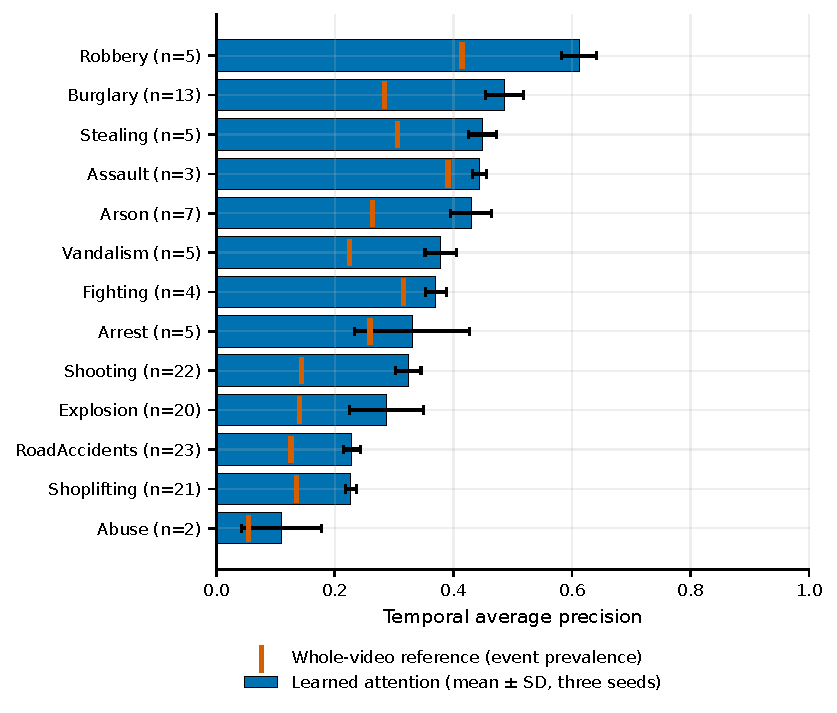
\includegraphics[width=0.9\textwidth]{fig_temporal_ap_by_category_r20.pdf}
    \caption[Temporal AP by anomaly category.]{Dense indexed temporal AP by anomaly category for the 135 source-bounded anomalous test videos (mean and sample SD over three seeds; $n$ is the number of videos). The orange mark is the whole-video reference, which equals the category's mean event prevalence. Most categories contain fewer than ten videos, so the ordering is not a ranking.}
    \label{fig:results-temporal-category}
\end{figure}


\end{appendices}
\newpage

%%%%%%%%%%%%%%%%%%%%%%%%%%%%%%%%%%%%%%%%%%%%%%%%%%%%%%%%%%%%%%%%%%%%%%%%%%%%%%%%%%%%%%%%%
\backmatter

% -- Bibliography
\printbibliography

% -- Eidesstattliche Erkl\"arung (= Affidavit)
% !TeX spellcheck = de_DE
% !TeX encoding = UTF-8

\chapter{Eidesstattliche Erkl\"arung}

	Hiermit versichere ich, dass ich diese \thesisType{} selbstst\"andig und ohne Benutzung anderer als der angegebenen Quellen und Hilfsmittel angefertigt habe und alle Ausf\"uhrungen, die w\"ortlich oder sinngem\"a\ss{} übernommen wurden, als solche gekennzeichnet sind, sowie, dass ich die \thesisType ~in gleicher oder \"ahnlicher Form noch keiner anderen Pr\"ufungsbeh\"orde vorgelegt habe.

	\vspace{3cm}

	Passau, \thedate

	\vspace{2cm}

	\parbox{8cm}{
		\hrule \strut \theauthor
	}



\end{document}
